%!TEX root = ../main.tex
%=========================================================

\section{Performance Evaluation}
\label{sec:eval}

%We evaluate the performance of \sysname prototype and answer the following research questions:
%\begin{enumerate} 
%    \item What is the overhead introduced by \sysname's register and lookup operations? %How does it compare to the current \discv system and vanilla DHT-based solutions?
%    What is the load distribution across network participants?
%    \item Does \sysname provide high performance for all the topics regardless of their popularity? 
%    \item How do malicious nodes impact \sysname's performance? How difficult is it to launch eclipse and DoS attacks against the system?
%\end{enumerate}

%We evaluate a prototype of \sysname to address the following research questions:
%\begin{enumerate} 
%    \item What is the overhead introduced by \sysname's register and lookup operations? How does the overhead of \sysname compare to the current \discv system and vanilla DHT-based solutions?
%    \item Does \sysname provide high performance for all the topics regardless of their popularity? What is the load distribution across network participants?
%    \item What is the impact of malicious nodes on \sysname’s performance? How difficult is it to launch various (\eg eclipse, DoS, \etc) attacks against the system?
%\end{enumerate}

%\subsection{Evaluation Setup}
%\para{Setup} 
We built a prototype of \sysname in PeerSim~\cite{p2p09-peersim}---a scalable P2P network simulator. In particular, we first implemented the Ethereum DHT by extending a vanilla Kademlia implementation~\cite{peersim_kademlia} with the required changes discussed in ~\Cref{sec:background:dht}. We then built \sysname on top of the Ethereum DHT implementation.

We compare \sysname against the following approaches:
\begin{enumerate}
\item \discv is the current discovery service~\cite{discv4} of Ethereum. In \discv, the DHT is merely used to perform \emph{random walks} in the P2P network. \er{not consistent with the presentation of discv4 as a collection of protocols before, see comments in intro.}
In \discv, a node issues three lookups to random destinations using  Kademlia lookup,  and it stores encountered nodes during the random walk in a buffer. The nodes in the buffer are consumed by the upper-layer Ethereum protocols (\eg RLPx~\cite{rlpx}) to make new connections, and when the buffer is empty new lookups are initiated to three other random nodes.
\item \altname is a traditional key/value store implementation using vanilla Kademlia DHT. 
In this approach, peers store their ads under desired topics at the N closest (by DHT distance metric) nodes to the corresponding topic hashes. In \altname, registrars accept all incoming ad registrations right away (\ie with no waiting time) and use a simple Last Recently Used (LRU) as a replacement policy.
\item \altnameticket is an extension of \altname. Unlike \altname, this approach uses \sysname's admission control mechanism (\Cref{sec:waitingTime}) to regulate the storage of incoming registrations. 
\end{enumerate}

%Both \altname and \altnameticket do not make use of a \emph{registration table} to keep track of on-going registrations and new registrations are periodically issued by nodes every advertisement period.


Many existing systems including the InterPlanetary File System (IPFS)---a decentralised content storage and sharing system---perform peer discovery using the \altname approach~\cite{libp2p_kaddht}. Therefore, we use \altname as a baseline solution in our experiments. 
As similarly done in the IPFS system, we use N=20 peers (\ie closest to the desired topic's hash) for storage of ads in both \altname and \altnameticket approaches.

% On the other hand, t
The topic lookup process in \altname and \altnameticket involve first finding N closest peers to the topic using the key lookup process of the Ethereum DHT as discussed in \Cref{sec:background:dht}. Once its lookup operation terminates with a stable list of closest peers to the desired topic, a searcher locally sorts those peers based on their distance (using Kademlia's XOR metric) to the topic's hash. Finally, the searcher queries $\alpha=3$ peers at a time, proceeding with the farthest to the closest of the N peers.

%On the other hand, the topic lookup for \altname and \altnameticket is similar to the \discv lookup.  When a node performs a lookup selects the 20 closest nodes to the topic hash from the local routing table and it sends topic query messages to the first  $\alpha=3$.
%In the reply, queried nodes attack the known nodes for the specific topic but also known nodes to the same distance of the topic hash. 
%The known nodes for the specific topic are stored in the lookup buffer. 
%The known nodes with the same distance to the topic id are added to the list of 20 closest nodes,  which is reordered and keeps only the 16 closest.
%The lookup process is ended when all 16 closest nodes are queried or when enough nodes are discovered for the queried topic, which is defined by the system parameter $N_\textit{lookup}$ 

\para{Metrics} The simulator reports the following performance metrics. 
 \begin{itemize}
     \item \textbf{Message Overhead} - the total number of messages received by each node. 
%We calculate separate values for both lookup and registration operations. 
Higher values mean larger strain put on each node. 
     \item \textbf{Discovered Peers} - the number of application-specific peers discovered by the searchers during lookup operations. This metric is a measure of the topic search performance by the peers.
%Each operation is finished after discovering 30 nodes. 
     \item \textbf{Discovered By} - the number of searchers each advertiser was discovered by. This metric allows us to verify whether each peer is being discovered and how the number of discoveries differs across peers.
%     \item \textbf{Registrations} - the number of registration placed by each advertiser and the number of registrations each  registrar accepted. It allows to verify the load on each registrar and analyse the their load distribution.
 \end{itemize}
 %We calculate per-node average for the metrics above and report their standard deviation.  Note that \emph{Discovered Peers} and \emph{Discovered By} metric will have the same average vales, but will vary in standard deviation. The same applies to \emph{Placed Registrations} and \emph{Accepted Registrations}. 
 
In the simulations, we verify the impact of the following parameters:
 \begin{itemize}
     \item \textbf{Network Size} - the total number of nodes that participate in the discovery. We set the default value to 25000, as similar number of live nodes were reported by the official Ethereum crawler~\cite{discv4-dns-lists} (\Cref{fig:ecosystem}). We assign each node an IP address and an ID from the crawled ENS records. \er{ENS records were never defined before.} We observe an average network churn of 3\% across daily crawls equal and therefore we use this value in our simulations to simulate nodes joining and leaving. 
     \item \textbf{Topics} - the number of distinct applications. We set the default number of topics to 300, which is similar to the observed value by the Ethereum crawler, and also experiment with values 100 and 600. To obtain the number of peers participating in each topic, we use a Zipf distribution with exponent $1.0$ (obtained empirically by fitting the crawler data, as shown in \Cref{fig:ecosystem}). 
     \item \textbf{Malicious nodes} - the number of attackers targeting the peers in the discovery system. We experiment with values ranging from 250 and 2500 nodes,  using 500 as the default value.  Each malicious node receives a distinct ID (\ie hash of its public key) generated following either uniformly at random or non-uniformly, \ie picking identifiers that are closer to the hash of the target topic than any honest node. The latter can be achieved in practice through ``brute-force'' generation of public keys until one with a suitable hash is found.
     \item \textbf{Malicious IPs} - the number of IP addresses available to all the attackers. We set its value between 1 and 100, using 10 for the default value. In our experiments, we use hypothetical attacker IP addresses that have minimum similarity with the set of real IP addresses used by IP addresses (obtained from the crawled ENS records) in order to obtain an upper-bound on the impact of attacks. %At the time of writing this paper, 99\% of the addresses in the Ethereum network are IPv4, and therefore we use only IPv4 addresses in the simulations.

%Meaning that every 25 malicious nodes will share a single, random IP address in the best case or every malicious node will use a different IP address in the worst case.  
 \end{itemize}


Each simulation takes one hour of simulated time during which each advertiser tries to maintain active (\ie unexpired) registrations and nodes each perform a single lookup operation uniformly spread across the simulation time.  For the \sysname and DHT-based solutions, we set the \emph{registration table} capacity to 500 to align with the memory requirements from the official Ethereum DHT implementation, and the ad expiration time is set to 15 min. % \ie every 15 min registration expires in the registrars. 

We set all the DHT-related parameters to the ones currently used by Ethereum DHT, \ie there are 17 buckets and up to 16 peers stored in each bucket.
Following Ethereum Kademlia specification,  each bucket has a replacement list of 10 nodes. 
Every 100 seconds a random bucket is checked for unresponsive nodes. 
If there are dead nodes, these are substituted by nodes from the replacement list.  If there are not enough nodes in the replacement list,  a new random lookup is performed to discover mode nodes.
Based on formal analysis (see \Cref{sec:analysis}), we set other \sysname parameters such as the number of registrations placed per bucket $K_{register}= 3$, the occupancy exponent $P_{occupancy} = 10$, the number of peers to contact per bucket during a topic lookup $L_\textit{lookup}=3$, the maximum number of ads a single registrar returns in a lookup $N_\textit{return}=10$. On the other hand, the total number of ads (\ie $N_\textit{lookup}$) is an application-specific parameter, which we set to 30 based on similar requirements of existing applications such as Geth.

%The values of these parameters were selected based on extensive simulations that we skip due to the space limitation but included in our Github repository~\cite{our_repo}. 

%%%%%%%%%%%%%%%%%%%%%%%%%%%%%%%%%%%%%%%%%%%%%%%%%%%%%%%%%%%
%\subsection{Message Overhead}
\subsection{Evaluation Results}

\para{Network performance}
In the rest of this section, we use violin plots for a compact illustration of both the distribution and the density of data points for each performance metric. For each plot, we limit the shape of the violins within the range of the observed data and set the widths of each data point in the violin proportional to the count of observations at that data point. 
Above a violin, we display the maximum observed values (vertically), if the range of the data points exceed the range of the y axis. 

%In~\Cref{fig:regMsgsPerTopic}~and~\Cref{fig:regMsgsPerSize},  we can observe the distribution of the total number of messages received per node related to the registration process, \ie registrations requests and replies during simulation time,  for different network sizes and different number of topics in the network.
%Both figures show no values for \discv protocol,  since  \discv nodes do not receive any registration message because they do not participate to any topic-based registration process.   \discv can only find nodes doing  \emph{random crawls} in the DHT  without being able to do topic specific queries. 
%
%\begin{figure}
%\centering
%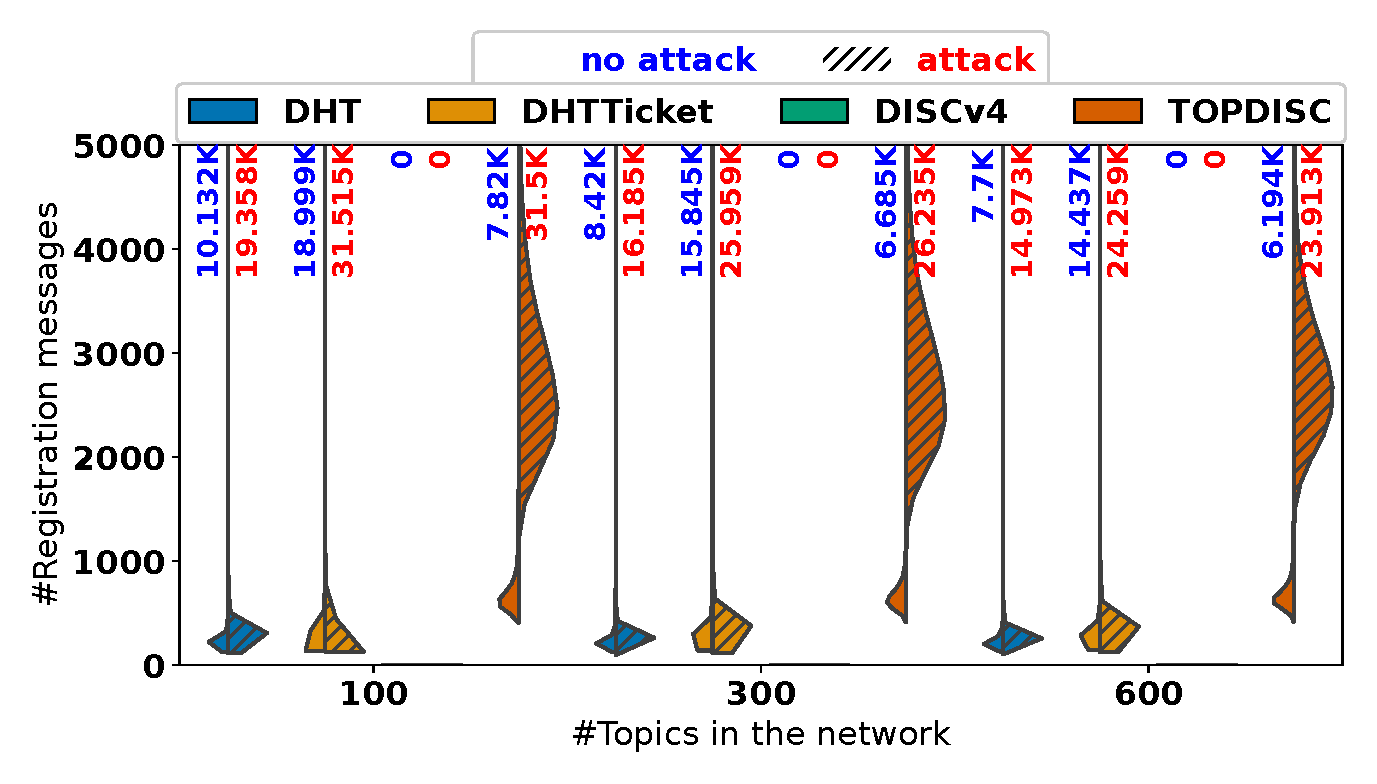
\includegraphics[width=\linewidth]{results/split/topic_registrationMsgs.eps}
%%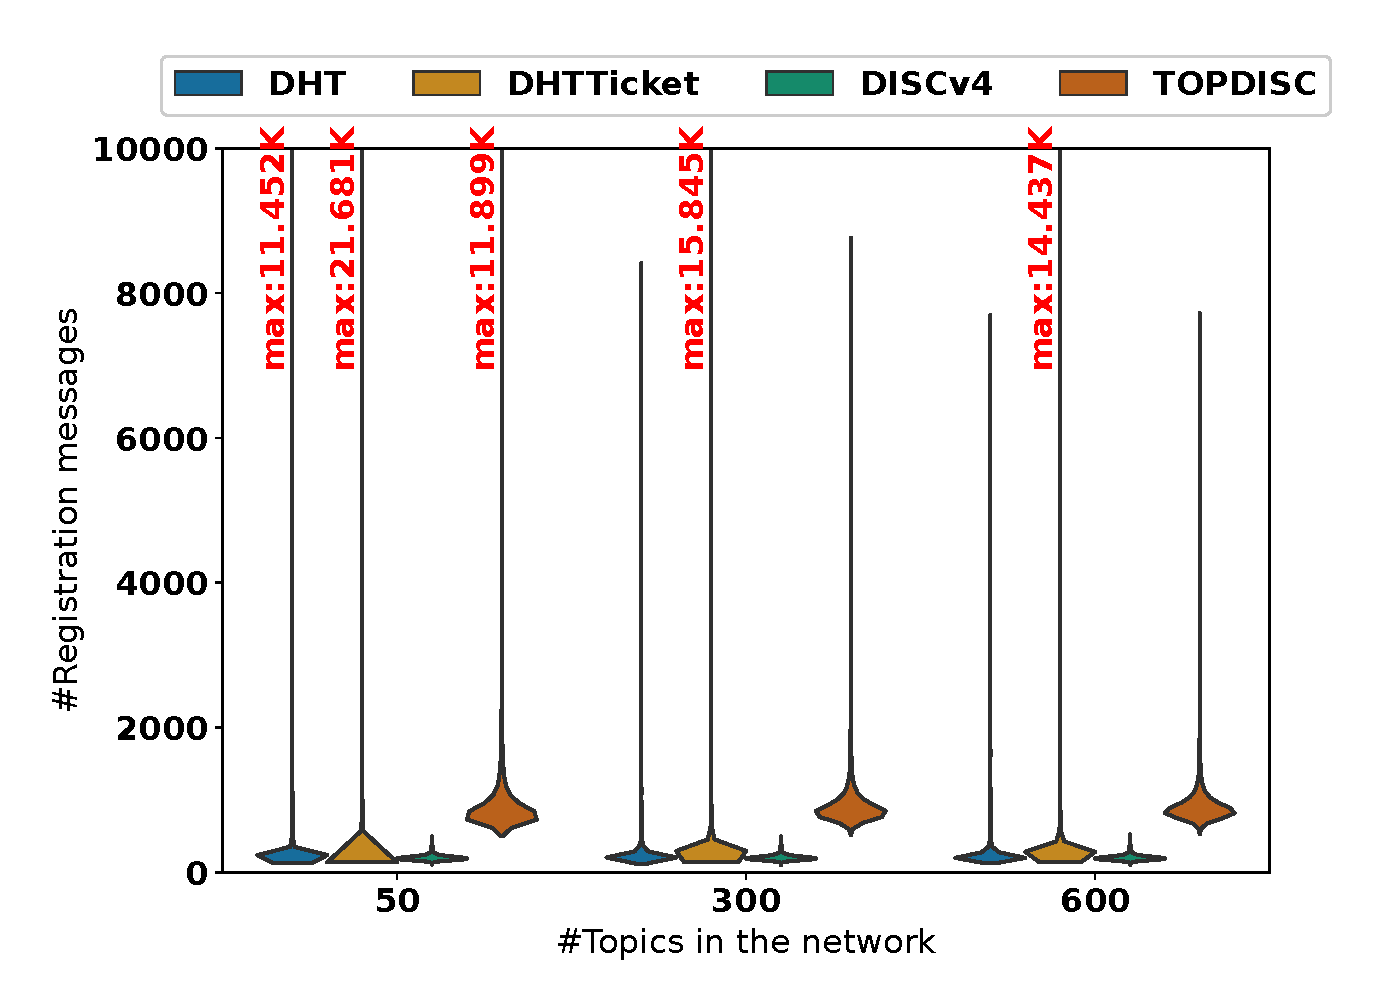
\includegraphics[width=\linewidth]{results/efficiency/violin_topic_registrationMsgs.eps}
%\caption{Y-axis: Distribution of registration related messages received by peers for varying number of topics for the simulation time.}
%\label{fig:regMsgsPerTopic}
%\end{figure}

%In~\Cref{fig:regMsgsPerTopic}~and~\Cref{fig:regMsgsPerSize},  we can observe while most of \sysname nodes receive around 500 registration messages,  with just a few receiving up to 5k messages in the worst case,  \altname solutions are more spread between 0 and 1000 received messages, but with some peaks up to 43k messages,  an order of magnitude higher than \sysname.
%This is caused by the fact that all nodes in \altname solutions try to put registrations starting by the closest nodes to the topic hash,  creating an uneven distribution  towards these nodes. 
%In \sysname, the use of \emph{advertise table} for advertisement placement provides a similar effect. 
%However this effect is diminished by the use of waiting times to regulate advertisement placement.  The increase of waiting time in the more congested nodes, causes that nodes starts more registrations in less congested nodes limiting the number of registrations placed on nodes close to topic hash.
%This effect is not seen when using \altname combined with tickets. 
%This is due to the fact that \altname is not using a \emph{advertise table} to keep track of ongoing registrations.  Because of this,  advertisers start new registrations towards the topic hash every advertisement period, even if they did not succeed in the previous attempts due to high waiting times.
%Therefore using tickets in the \altnameticket, maybe useful to increase the diversity in the \emph{advertise tables} but not for load balancing between nodes.
%
%When increasing the number of topics in the network (\Cref{fig:regMsgsPerTopic}), it is not observed an increase of registration messages for any of the different protocols. 
%However,  when increasing the number of nodes participating in the network (\Cref{fig:regMsgsPerSize}),  also registrations messages received per nodes are increased, as expected.
%But this increase is very different between \sysname and \altname protocols.
%\sr{tbc with specific values}

%\begin{figure}[!h]
%\centering
%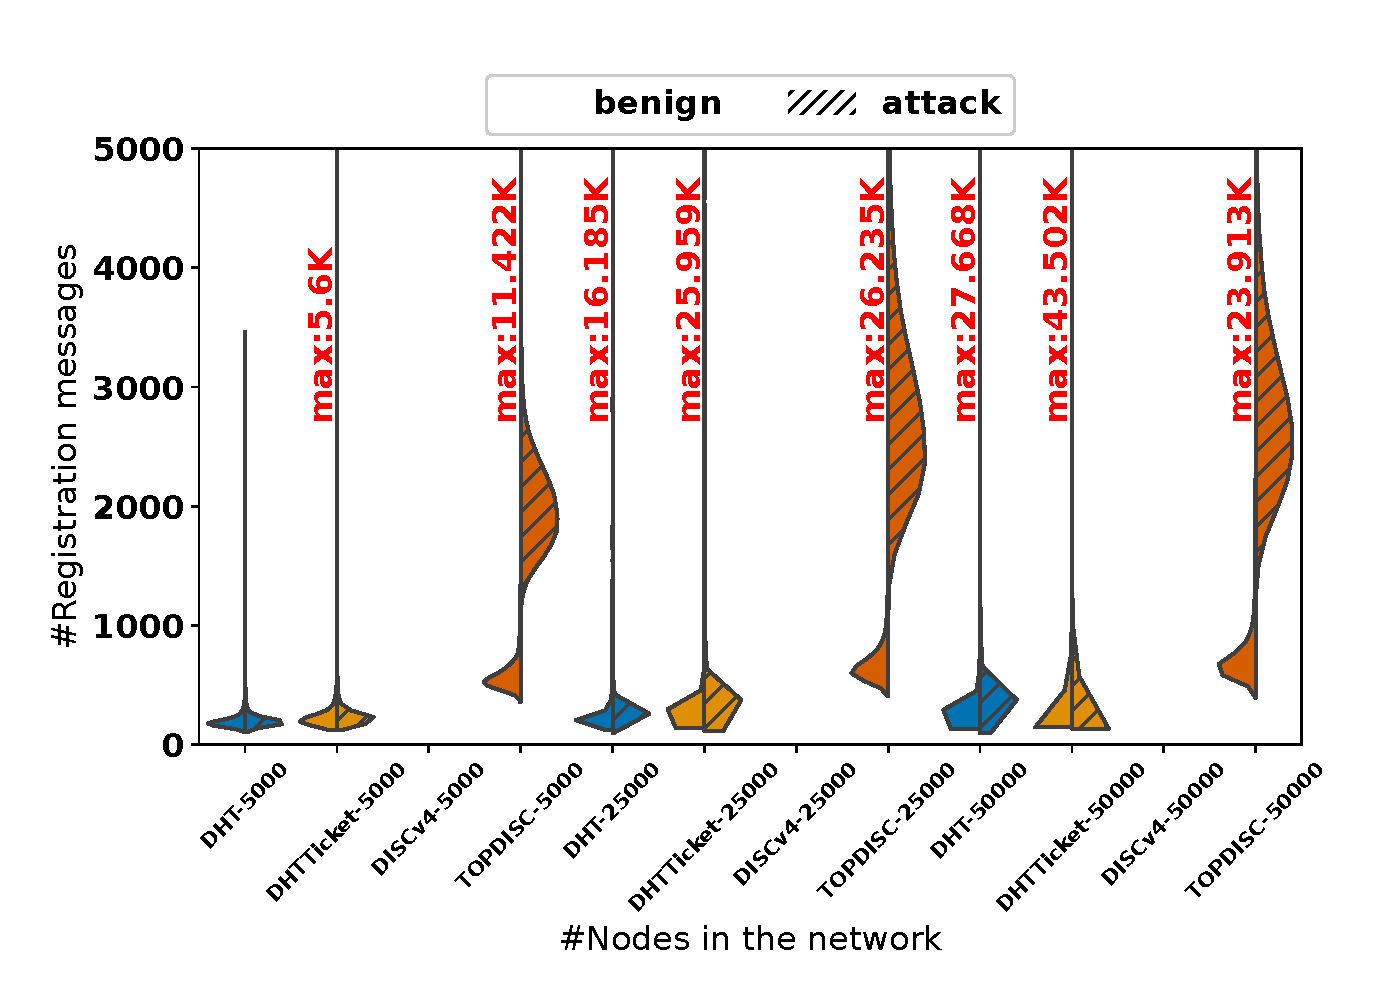
\includegraphics[width=\linewidth]{results/split/size_registrationMsgs.eps}
%%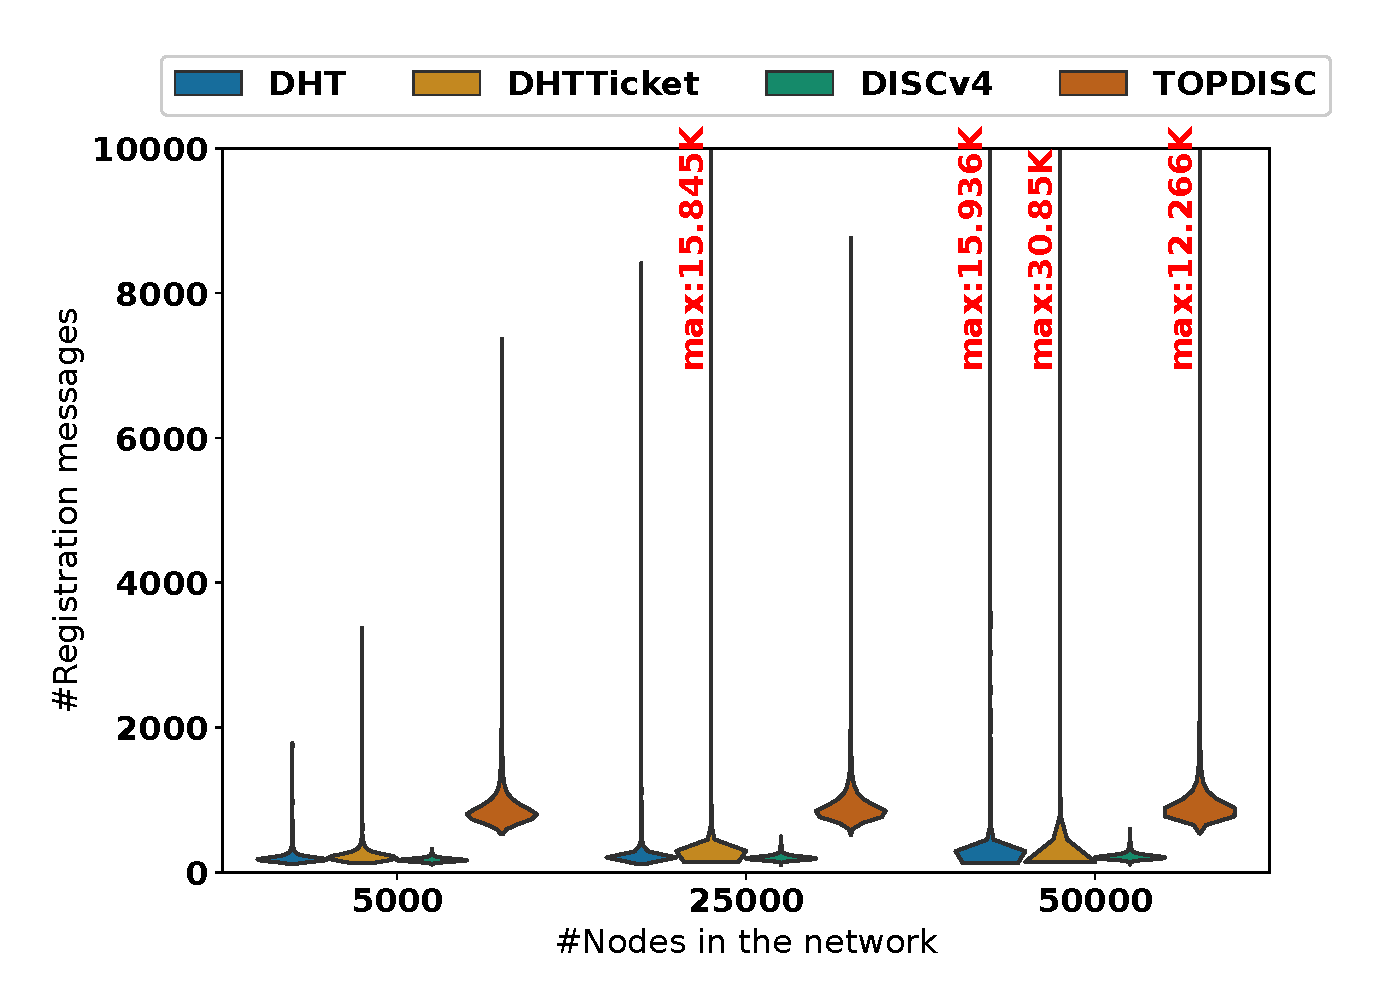
\includegraphics[width=\linewidth]{results/efficiency/violin_size_registrationMsgs.eps}
%\caption{Y-axis: Distribution of registration related messages received by peers for different network size for the simulation time.}
%\label{fig:regMsgsPerSize}
%\end{figure}
%
%\begin{figure}
%\centering
%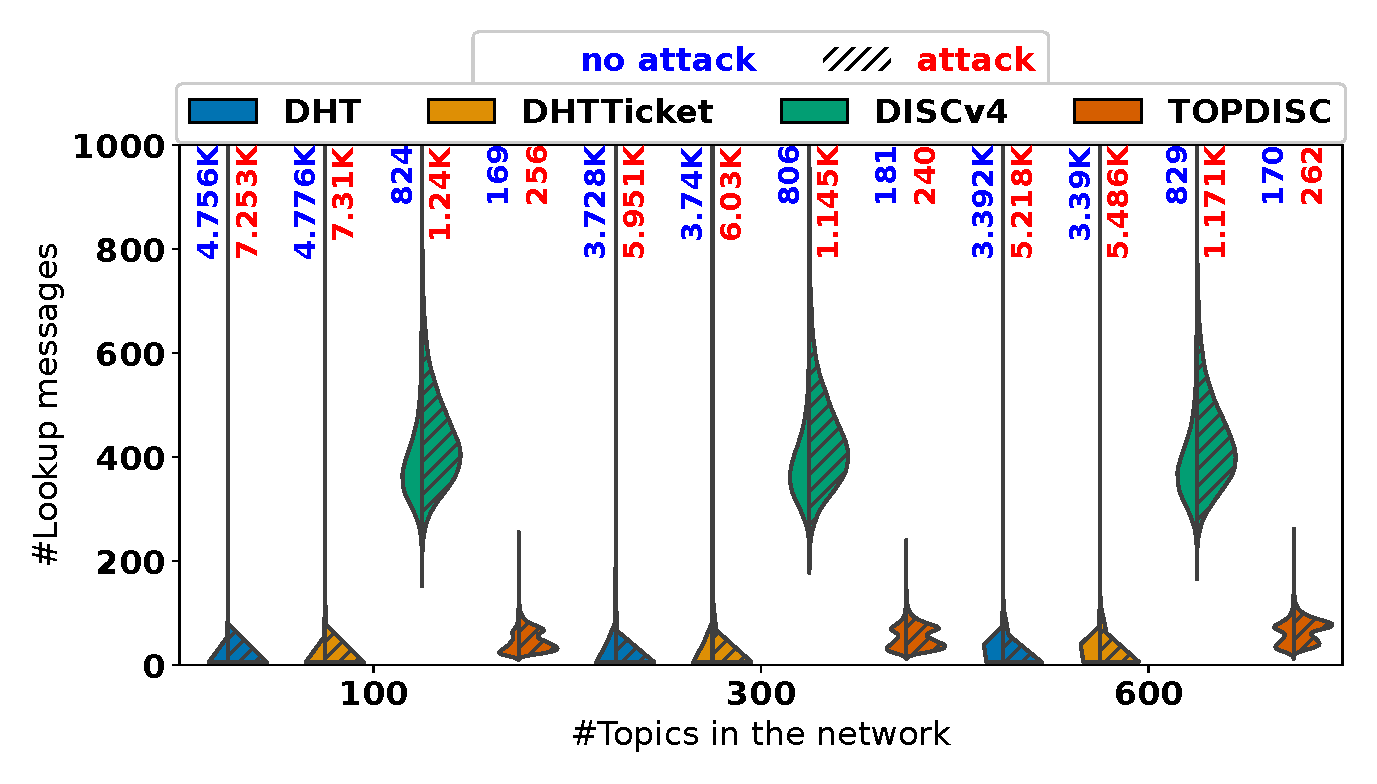
\includegraphics[width=\linewidth]{results/split/topic_lookupMsgs.eps}
%%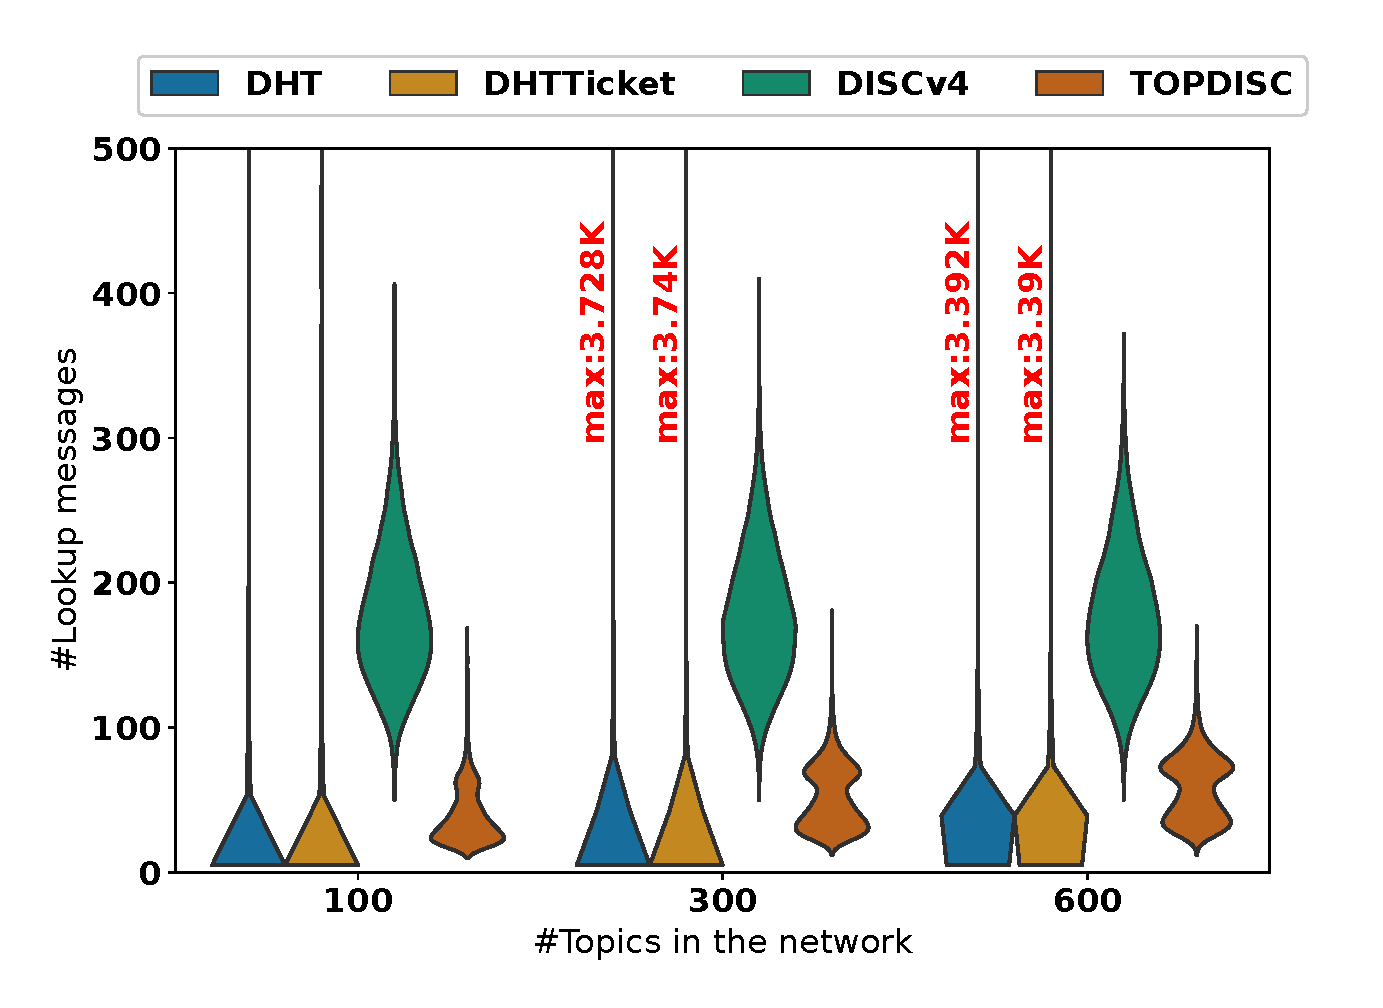
\includegraphics[width=\linewidth]{results/efficiency/violin_topic_lookupMsgs.eps}
%\caption{Y-axis: Distribution of lookup messages received by peers for varying number of topics for the simulation time.}
%\label{fig:lookupMsgPerTopic}
%\end{figure}
%
%\begin{figure}[!h]
%\centering
%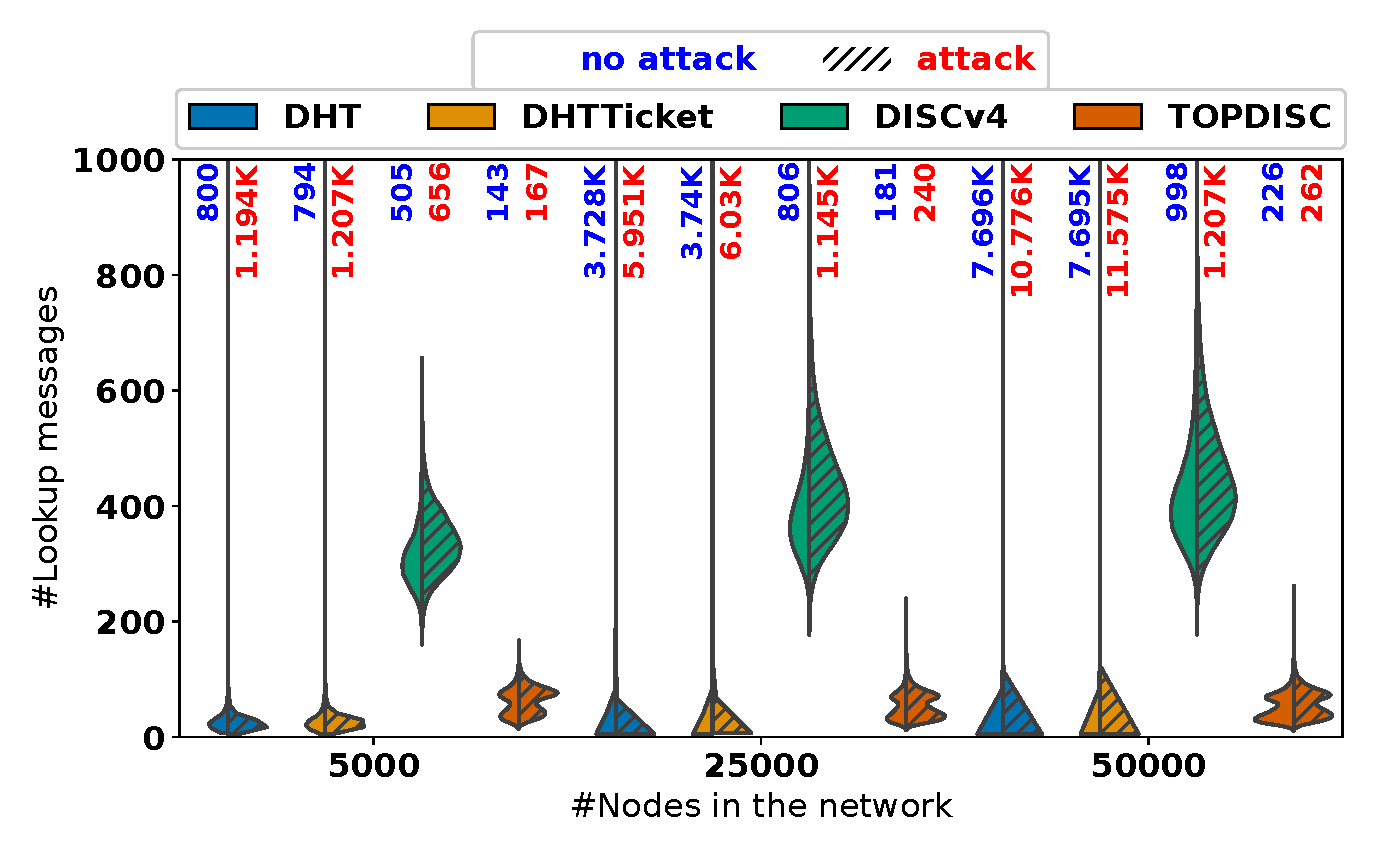
\includegraphics[width=\linewidth]{results/split/size_lookupMsgs.eps}
%%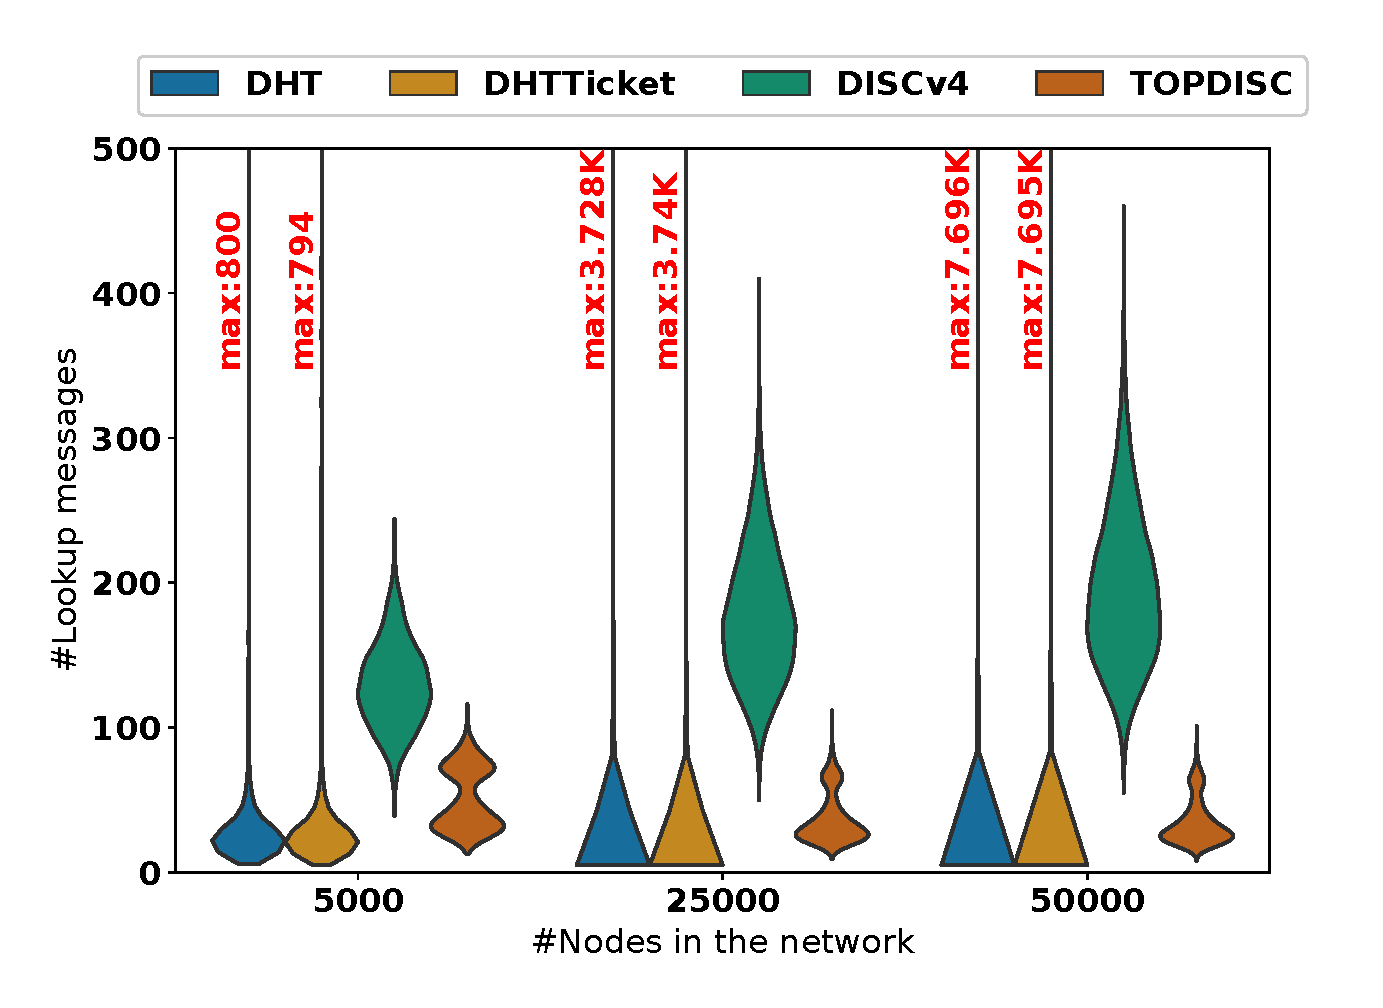
\includegraphics[width=\linewidth]{results/efficiency/violin_size_lookupMsgs.eps}
%\caption{Y-axis: Distribution of lookup messages received by peers for different network size for the simulation time.}
%\label{fig:lookupMsgPerSize}
%\end{figure}

%In~\Cref{fig:lookupMsgPerTopic}~and~\Cref{fig:lookupMsgPerSize}, we observe the number of messages related to the lookup process, \ie topic queries and replies for \sysname, \altname and \altnameticket, and kademlia find/response messages for \discv. We evaluated using  different network sizes and different number of topics in the network. 
%There is a single lookup in the simulation per node, and the $N_\textit{lookup}$ parameter used is equal to 30.  Therefore nodes stop the lookup process when found 30 different nodes in the network for the intended topic.
%In the figures we can observe there is a big different between topic-aware protocols (\sysname, \altname and \altnameticket) and \discv. 
%
%\sr{why there is an increase for \discv with the number of nodes in the simulation and not the number of topics??? shouldn't be the opposite? I guess is because even if there are topics with less nodes there is just a single lookup with the same nodes contacted}
%\sr{why the peak is bigger for DHT for 600 than 300? Is it because of topic hash ids colliding?}

\begin{figure}[!h]
\centering
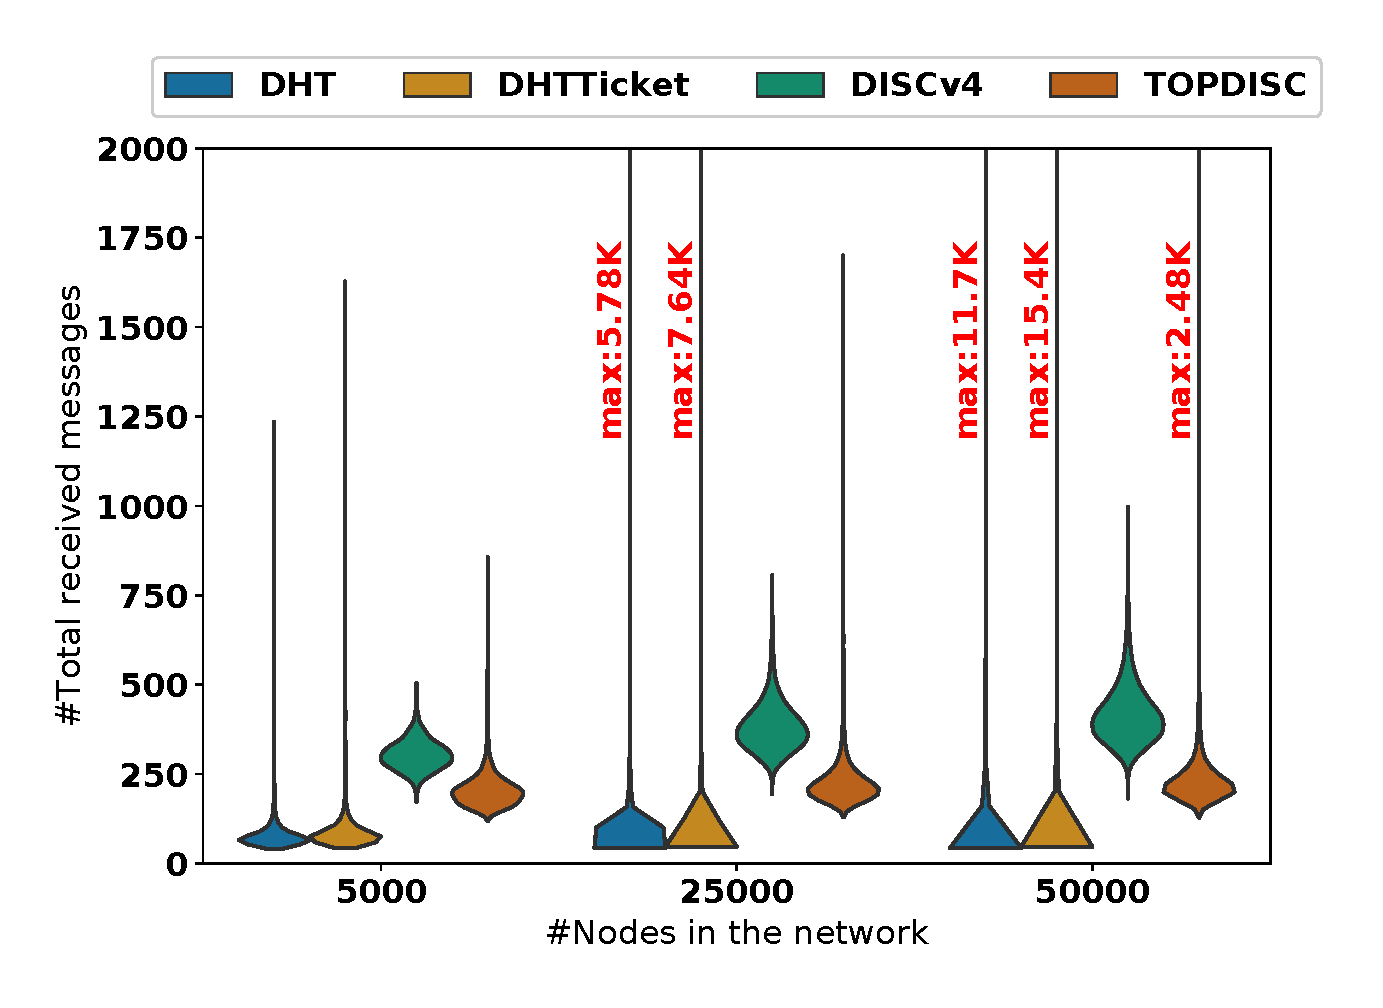
\includegraphics[width=0.470\textwidth]{results/no_split/violin_size_totalMsg.eps}
%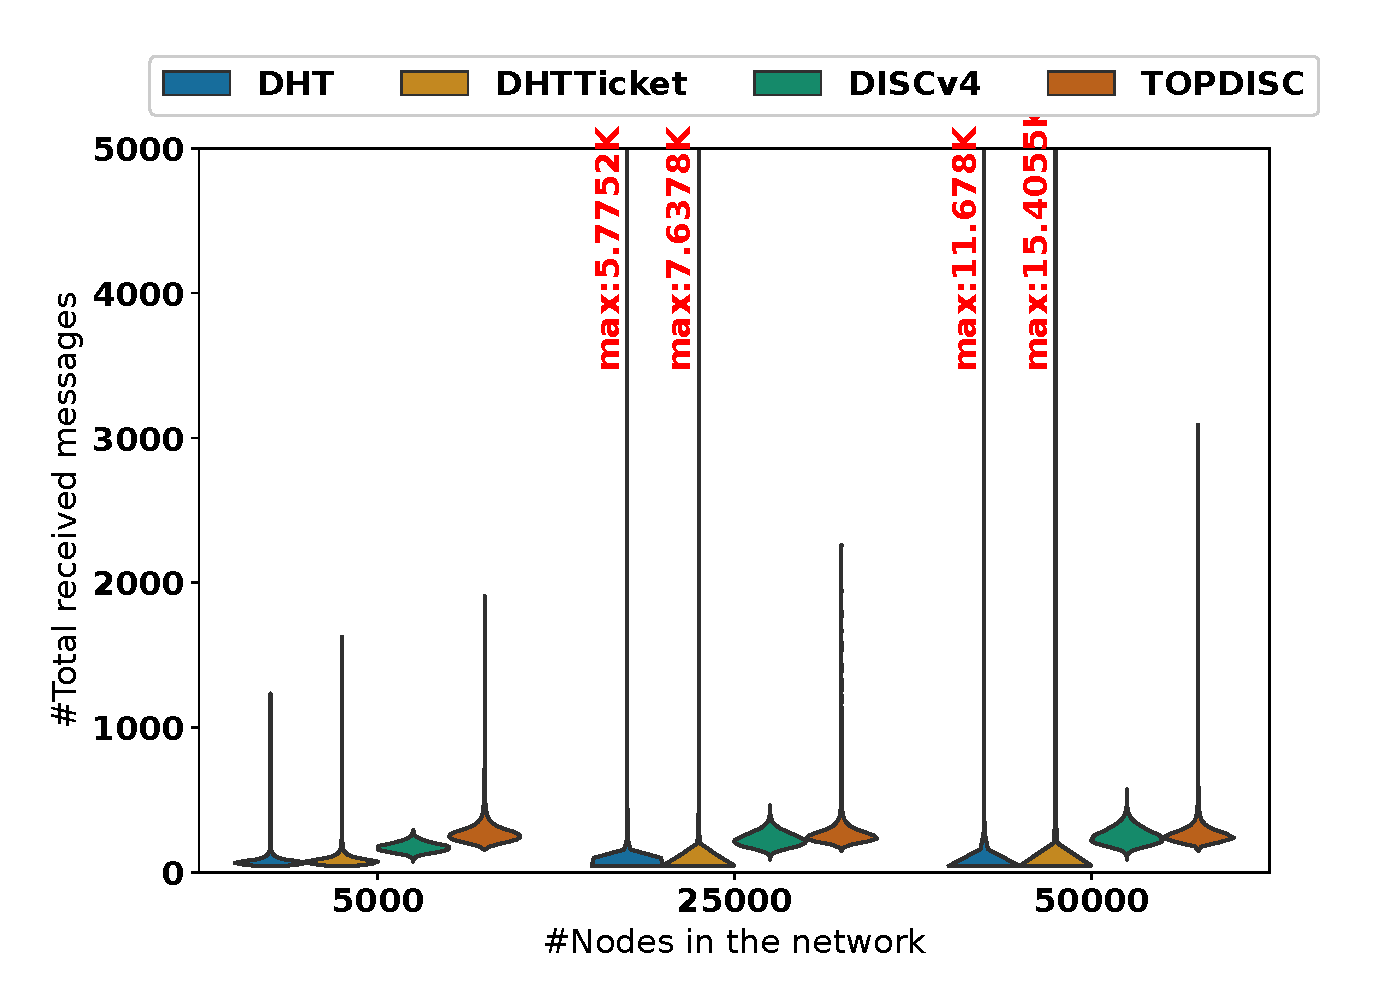
\includegraphics[width=\linewidth]{results/efficiency/violin_size_totalMsg.eps}
\caption{Y-axis: Distribution of discovery related (including registration and lookup) messages received by peers for different network size during a single advertisement period.}
\label{fig:msgsPerSize}
\vspace{-0.15in}
\end{figure}

\begin{figure}
\centering
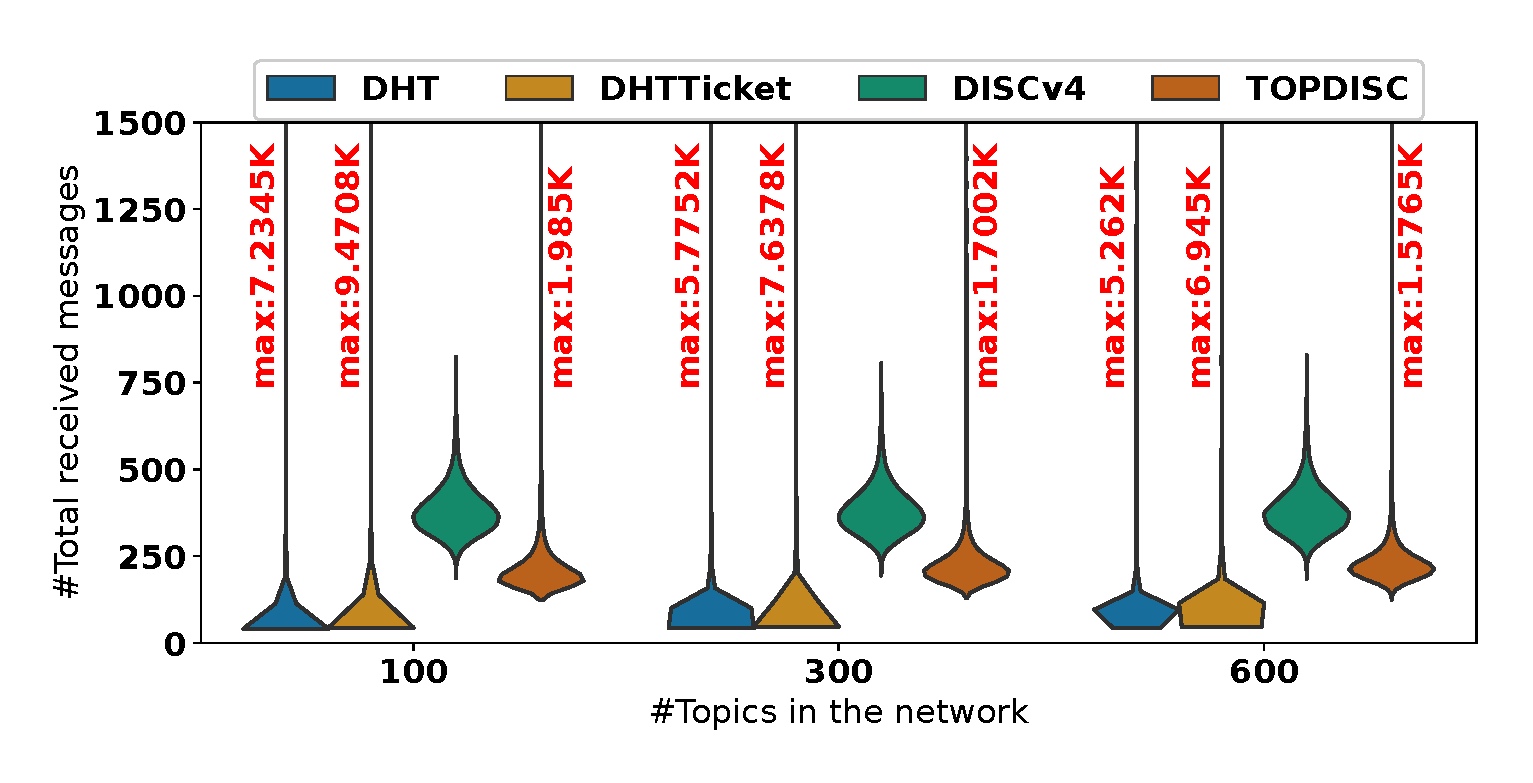
\includegraphics[width=0.470\textwidth]{results/no_split/violin_topic_totalMsg.eps}
%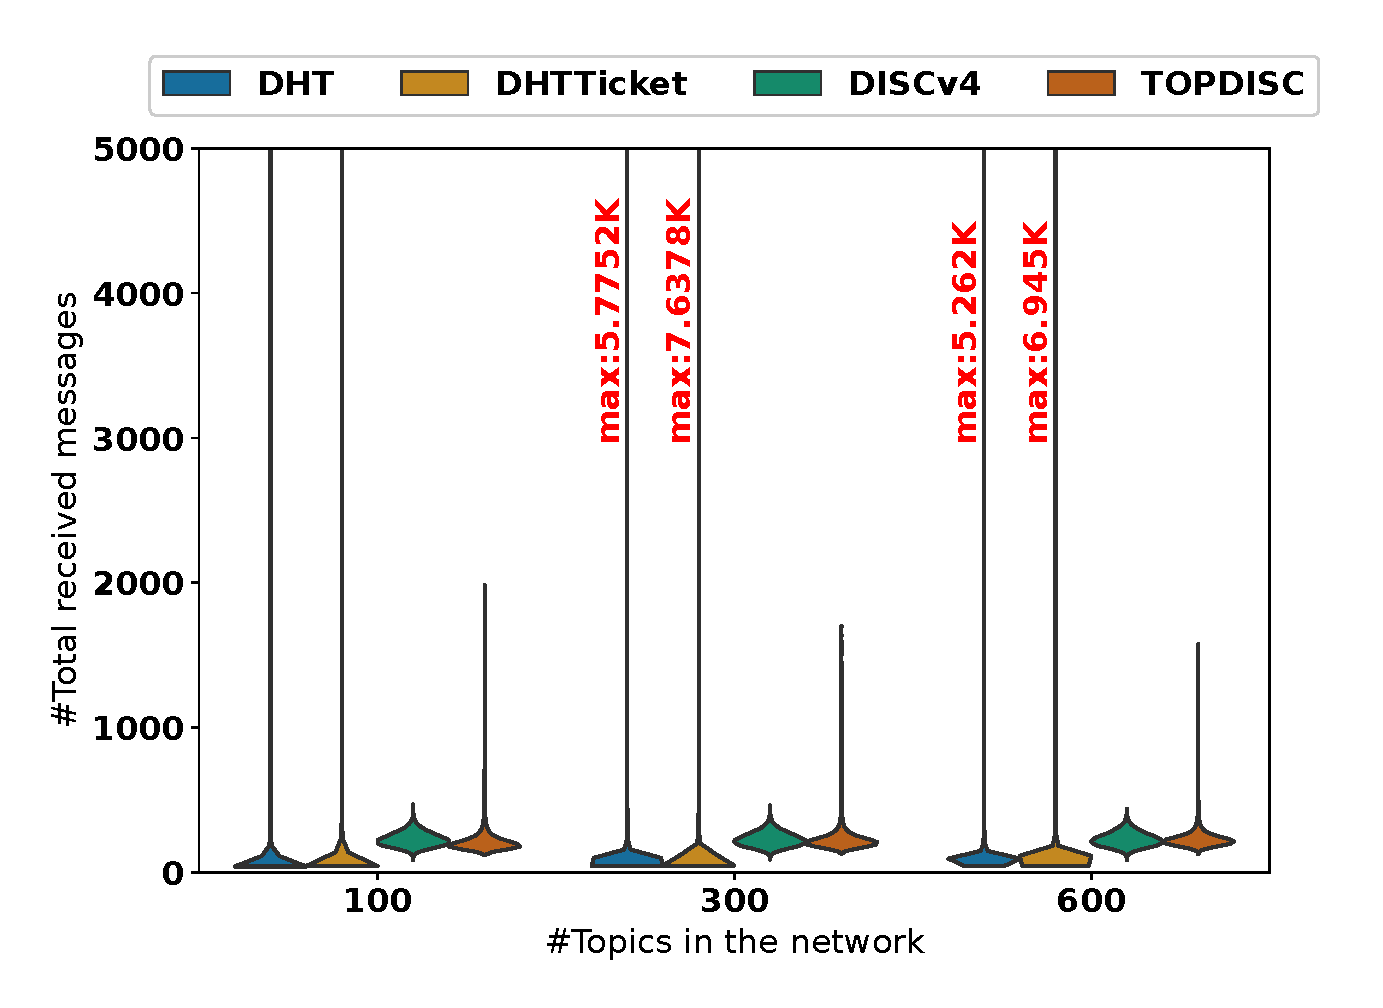
\includegraphics[width=\linewidth]{results/efficiency/violin_topic_totalMsg.eps}
\caption{Y-axis: Distribution of discovery related (including registration and lookup) messages received by peers for different number of topics during a single advertisement period.}
\label{fig:msgsPerTopic}
\vspace{-0.15in}
\end{figure}

In~\Cref{fig:msgsPerSize}~and~\Cref{fig:msgsPerTopic}, we present the total number of received messages (\ie overhead) received by the nodes as part of registration and lookup processes. For \discv, only lookups generate messages as there is no registration process in the protocol.
We observe the total number of messages during the simulation but averaged over ad expiration periods (\ie 15 minutes long). Therefore, the message counts relate to a single lookup followed by a single registration process per node before advertisements expire and are refreshed again. \er{consider revising this paragraph for clarity}

We observe that \altname protocols have poor fairness and scalability since the number of messages received by the nodes close to each topic hash increases linearly both 
% with increase 
in the number of nodes and topics. 
The \discv protocol has a better load distribution between nodes. since the destination of lookup messages is chosen randomly. However, the average load across nodes in \discv is the highest among all protocols, because nodes have to query a large number of peers during a lookup before they can discover sufficient number of topic-specific peers.
%, increasing the overhead during lookup.
\sysname, in comparison, provides significantly lower overhead.
% than the other protocols. 

%%%%%%%%%%%%%%%%%%%%%%%%%%%%%%%%%%%%%%%%%%%%%%%%%%%%%%%%%%%
%\subsection{Lookup performance}

\begin{figure}[!h]
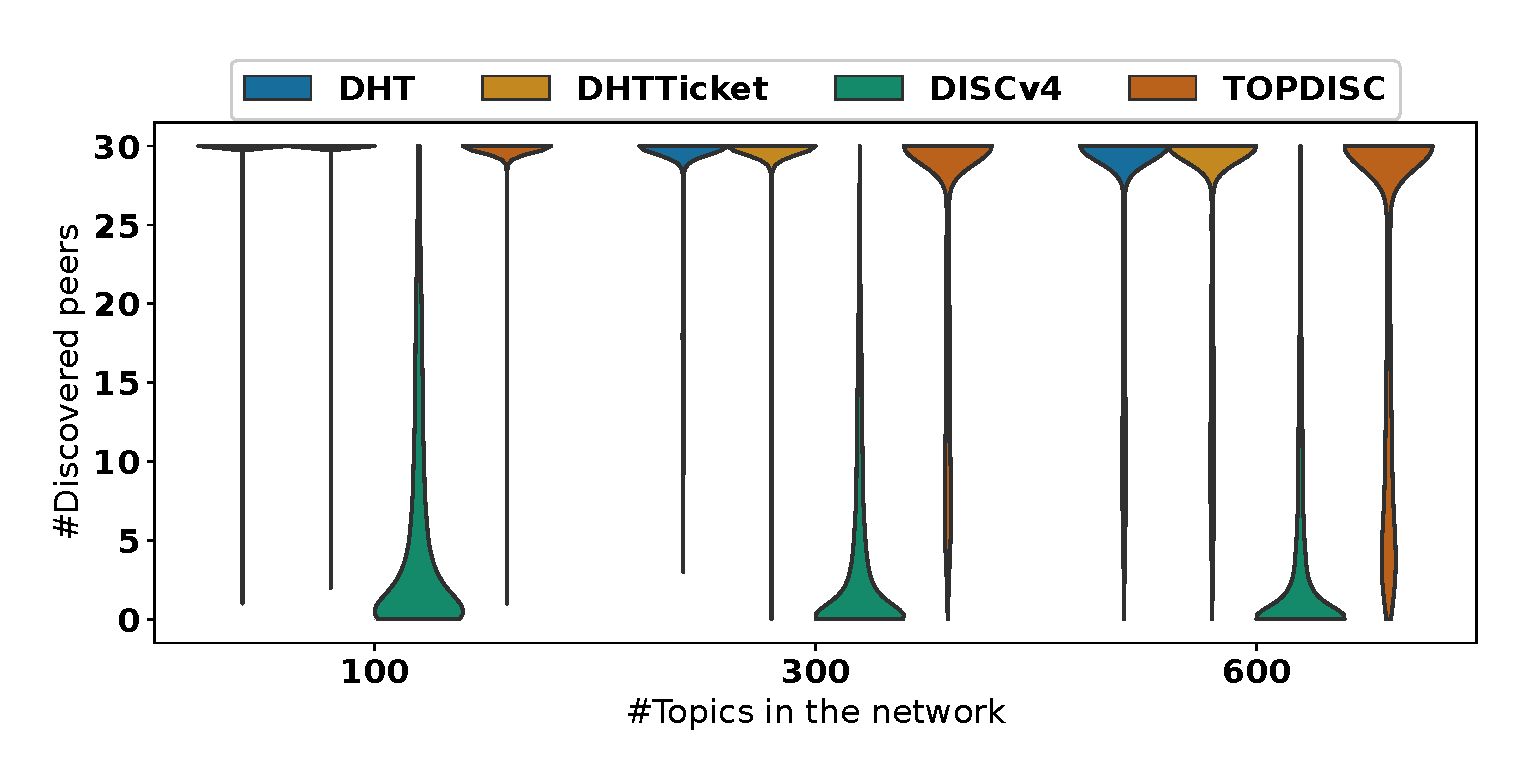
\includegraphics[width=0.470\textwidth]{results/no_split/violin_topic_discovered.eps}
%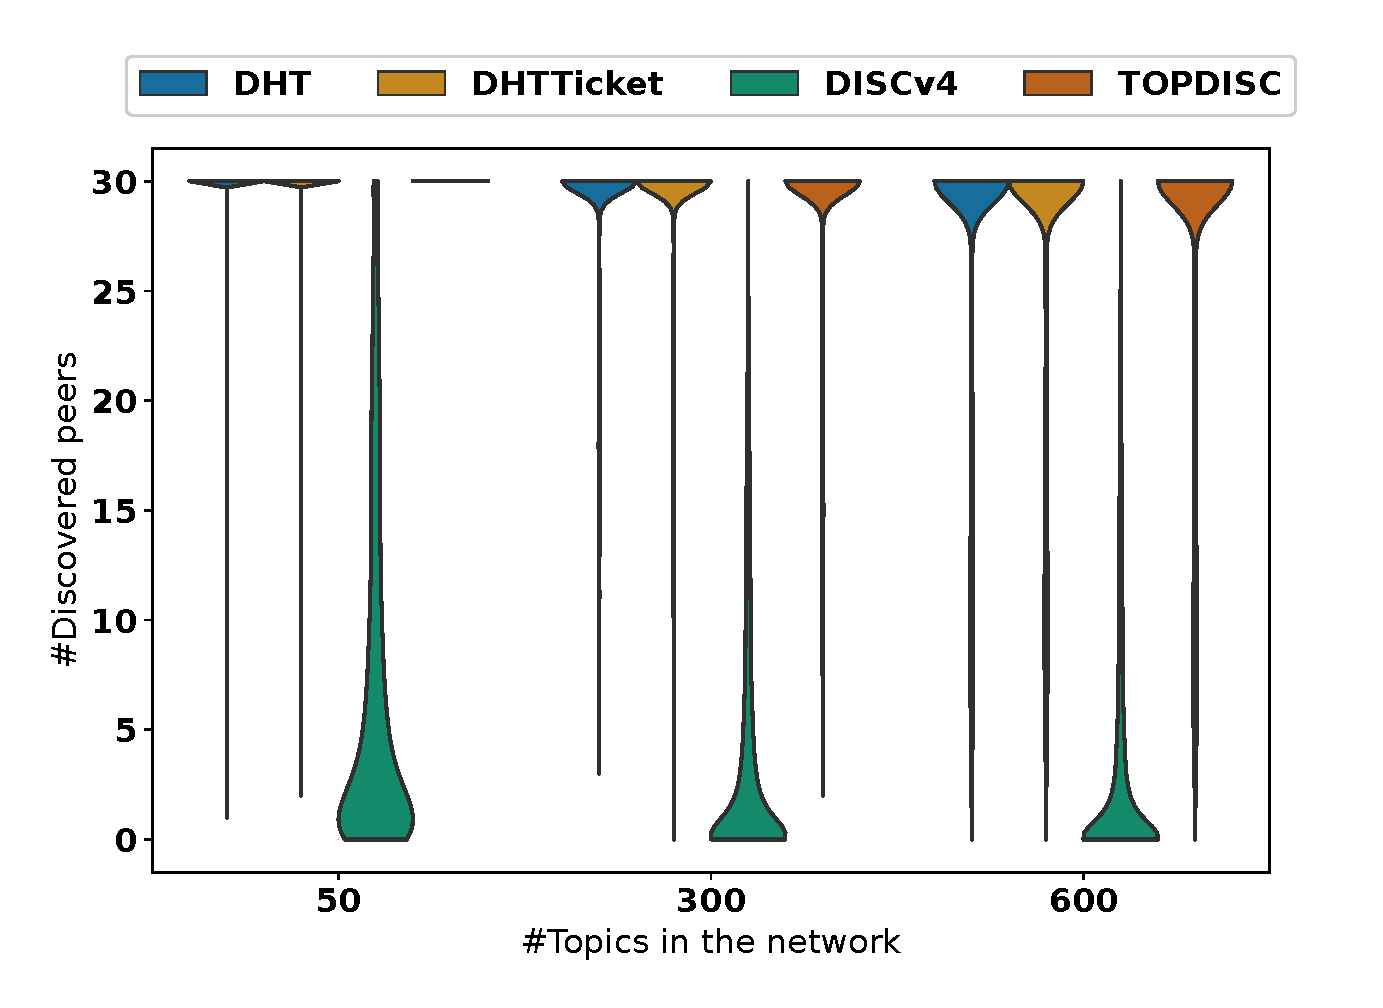
\includegraphics[width=\linewidth]{results/efficiency/violin_topic_discovered.eps}
\vspace{-0.05in}
\caption{Y-axis: Distribution of the number of peers discovered during lookup operation for different number of topics.}
\label{fig:discoveredPerTopic}
\vspace{-0.20in}
\end{figure}

\Cref{fig:discoveredPerTopic} presents the number of peers discovered during a single lookup operation with an increasing number of topics in the network. We observe that, in \discv, nodes discover a much lower number of application-specific peers per operation, while \sysname and DHT-based solutions efficiently discover the required (30) amount of peers to terminate the lookup. In rare cases, \sysname and DHT-based solutions do not discover the required amount of peers that are caused by unpopular topics with close to 30 participants. 
DHT-based solutions, \altname and \altnameticket, demonstrate the best discovery performance since searchers directly query the nodes, close to their target topic, where registrations from all application-specific peers are stored. Finally, we observe that \sysname achieves very close lookup performance to DHT protocols. 

%\michal{regarding \Cref{fig:discoveredPerTopic}, it seems that for 300 and 600 topics, we discover slightly less peers on average than the DHT solutions. Why is that? Those results should be for the same topic distributions across protocols, right?}
%\sergi{I think is normal and is caused by the fact that dht is going straight to nodes with most of the registrations so, specially with topics with very few nodes, they can find nodes faster, but with the tradeoff of being eclipsed very easy.}

\begin{figure}[!h]
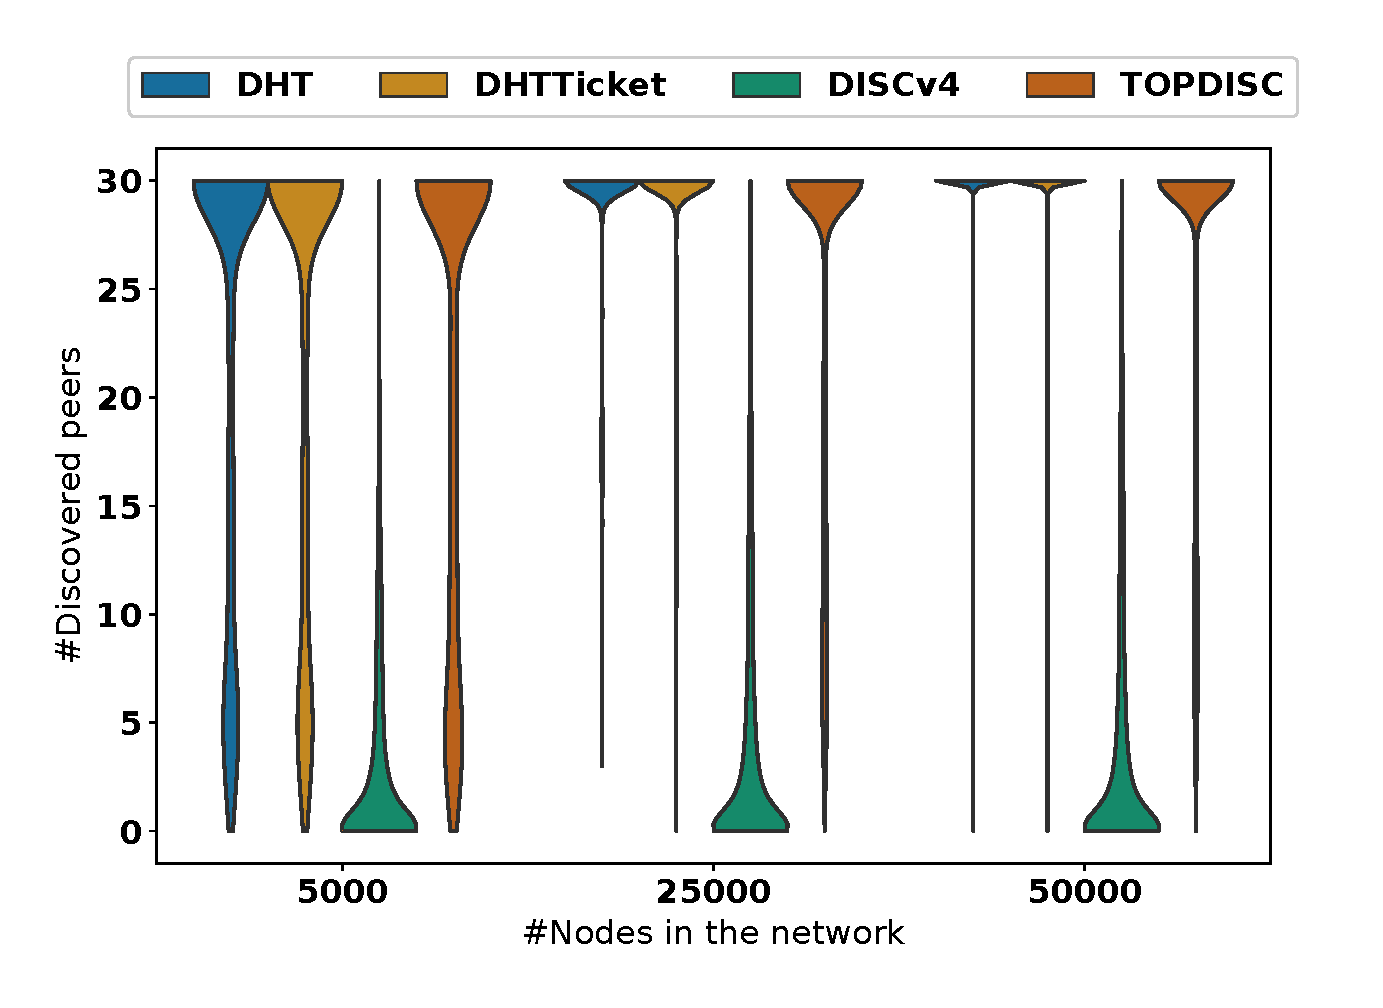
\includegraphics[width=0.470\textwidth]{results/no_split/violin_size_discovered.eps}
%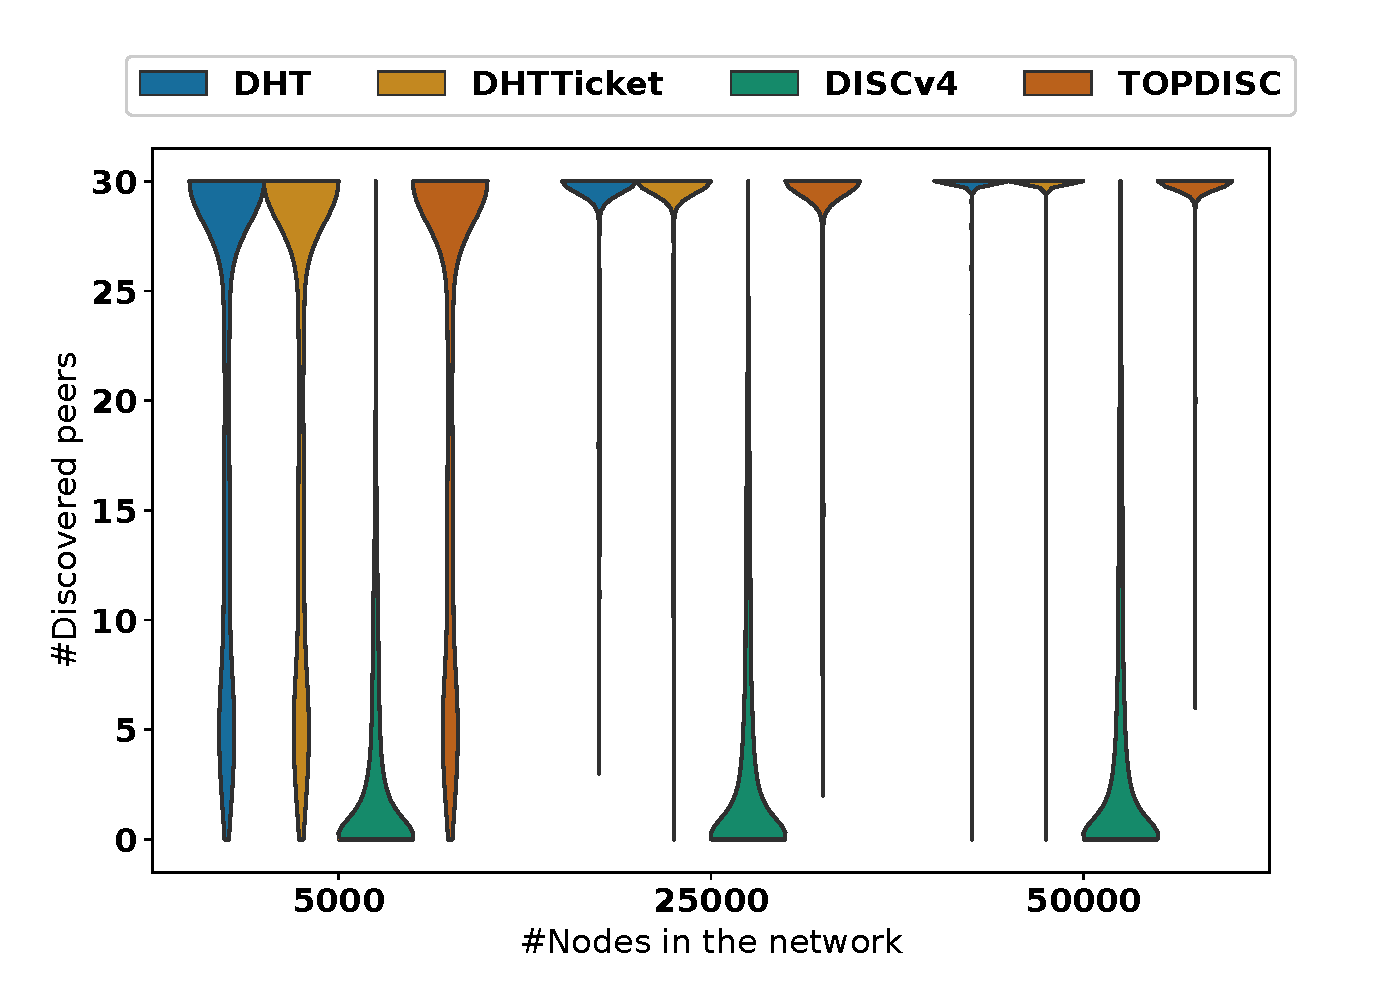
\includegraphics[width=\linewidth]{results/efficiency/violin_size_discovered.eps}
\caption{Y-axis: Distribution of the number of peers discovered during lookup operation for different network size.}
\label{fig:discoveredPerSize}
\vspace{-0.20in}
\end{figure}

\Cref{fig:discoveredPerSize} presents the number of peers discovered during a single lookup operation with an increasing network size. With a fixed amount of topics, each application-specific network grows and for all the protocols, it is easier to find the required amount of nodes.
 However, \discv again suffers from poor performance for all the investigated network sizes. 

\iffalse %Onur: removing these for now
\begin{figure}
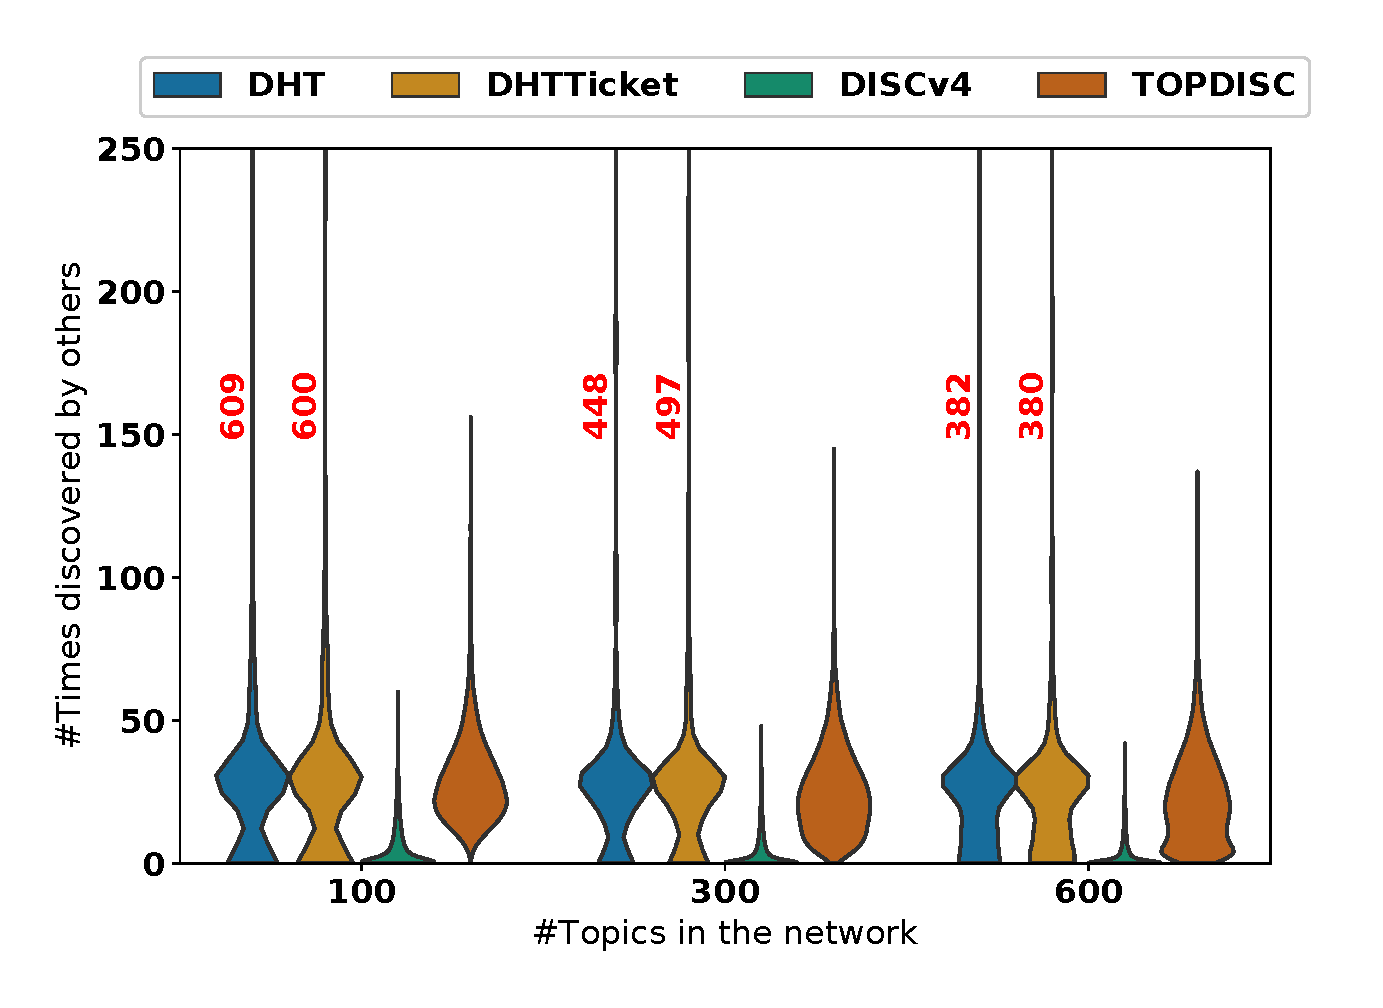
\includegraphics[width=0.470\textwidth]{results/no_split/violin_topic_wasDiscovered.eps}
%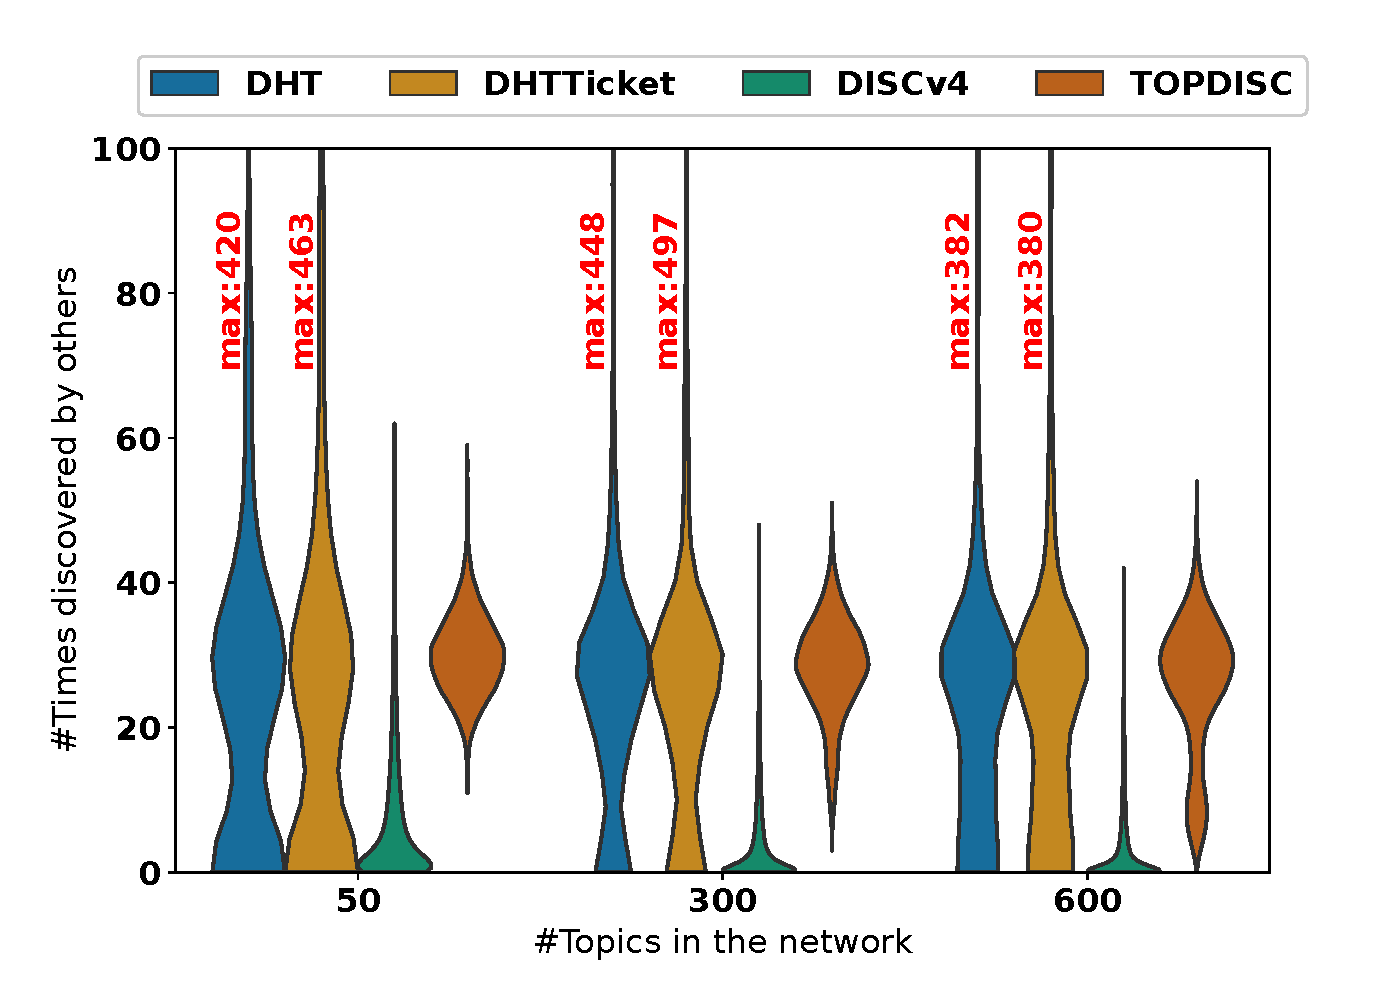
\includegraphics[width=\linewidth]{results/efficiency/violin_topic_wasDiscovered.eps}
\caption{Y-axis: Distribution of the number of times a peer is discovered by others for number of topics in the network for the simulation time.}
\label{fig:discoveredByPerTopic}
\vspace{-0.20in}
\end{figure}

\begin{figure}[!h]
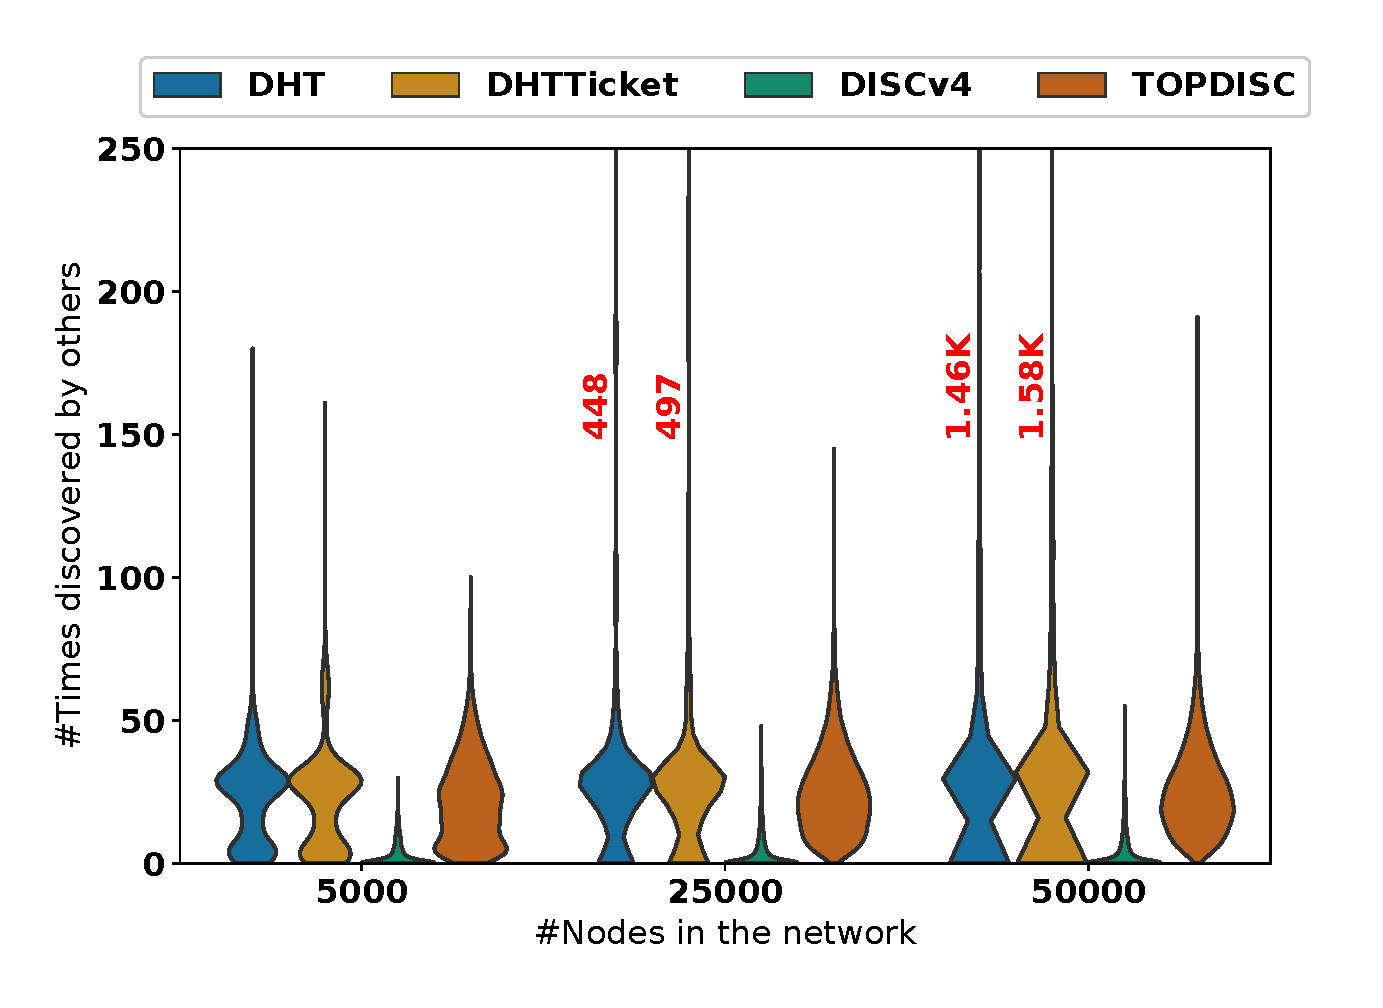
\includegraphics[width=0.470\textwidth]{results/no_split/violin_size_wasDiscovered.eps}
%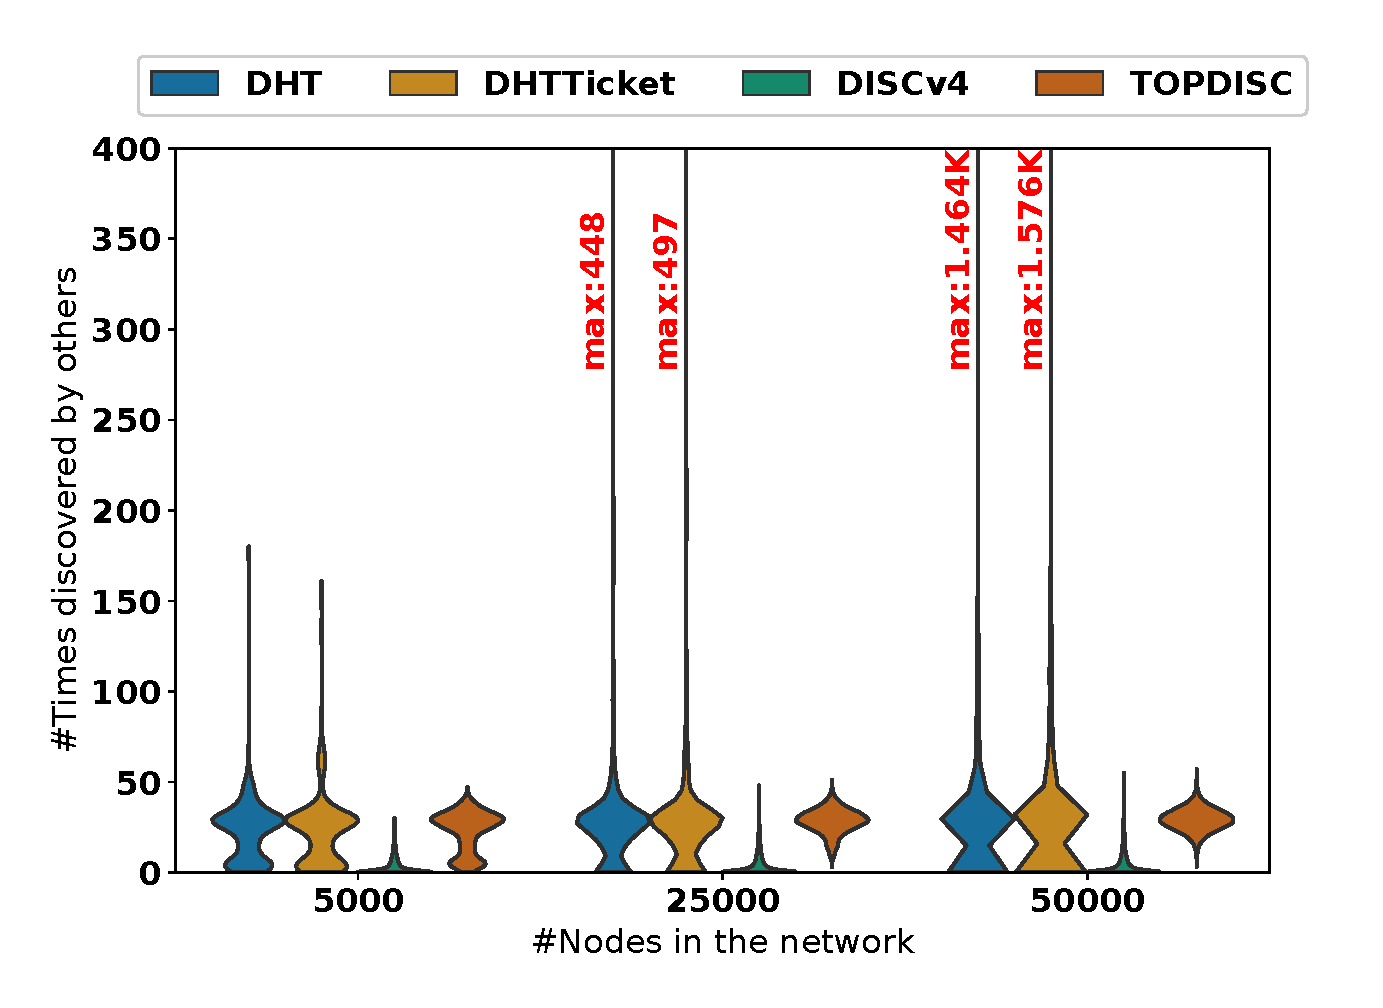
\includegraphics[width=\linewidth]{results/efficiency/violin_size_wasDiscovered.eps}
\caption{Y-axis: Distribution of the number of times a peer is discovered by others for different network size for the simulation time.}
\label{fig:efficiency_size}
\end{figure}
\fi 
%\subsection{Registrations}
%
%
%\begin{figure}
%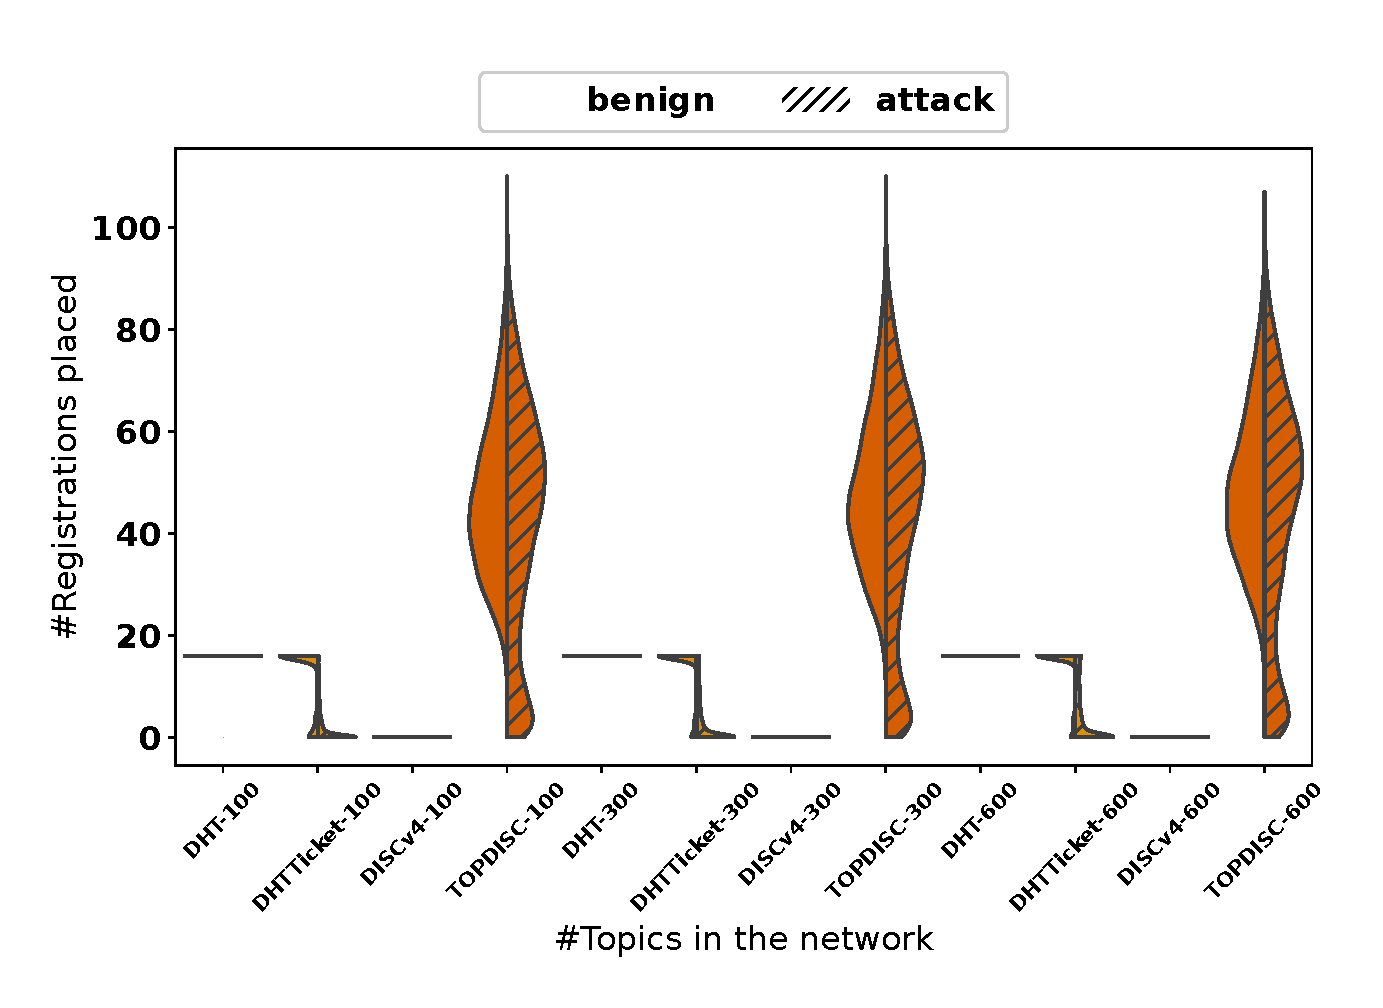
\includegraphics[width=\linewidth]{results/split/topic_regsPlaced.eps}
%%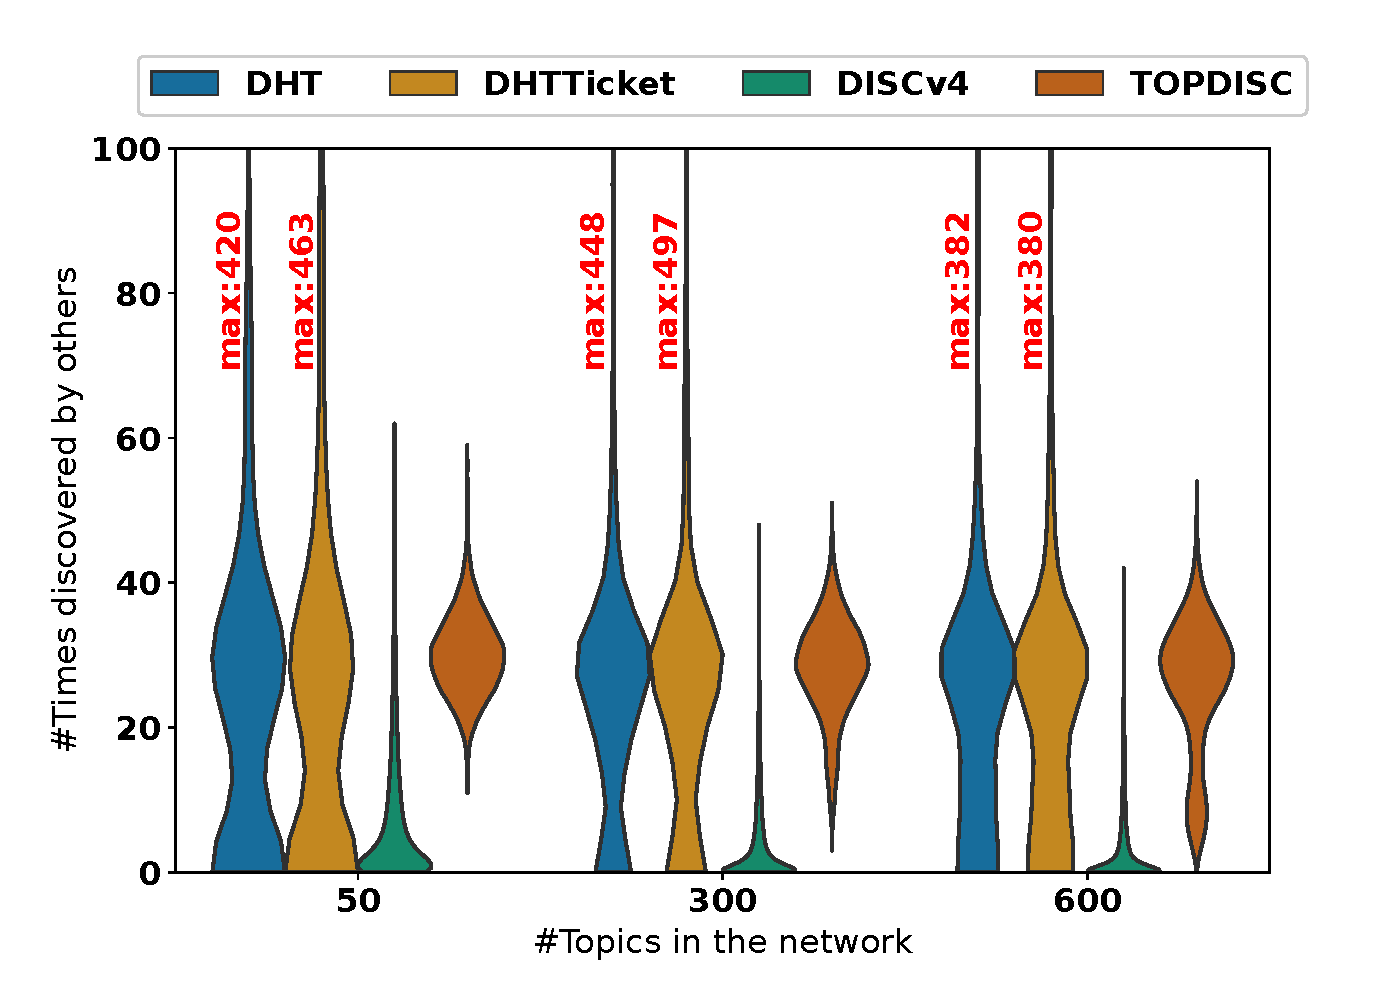
\includegraphics[width=\linewidth]{results/efficiency/violin_topic_wasDiscovered.eps}
%\caption{Y-axis: .}
%\label{fig:regsPlacedPerTopic}
%\end{figure}
%
%\begin{figure}[!h]
%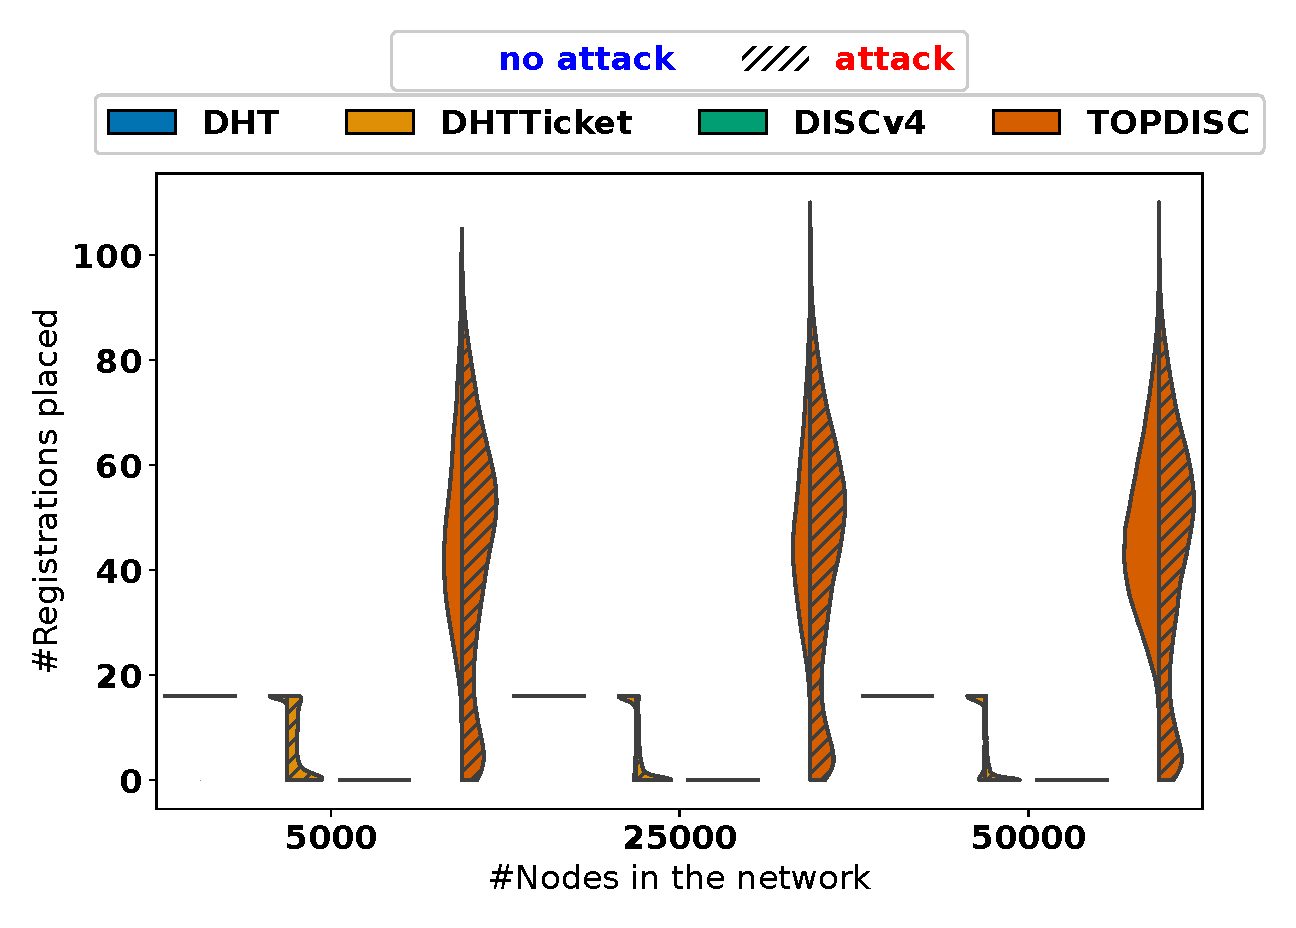
\includegraphics[width=\linewidth]{results/split/size_regsPlaced.eps}
%%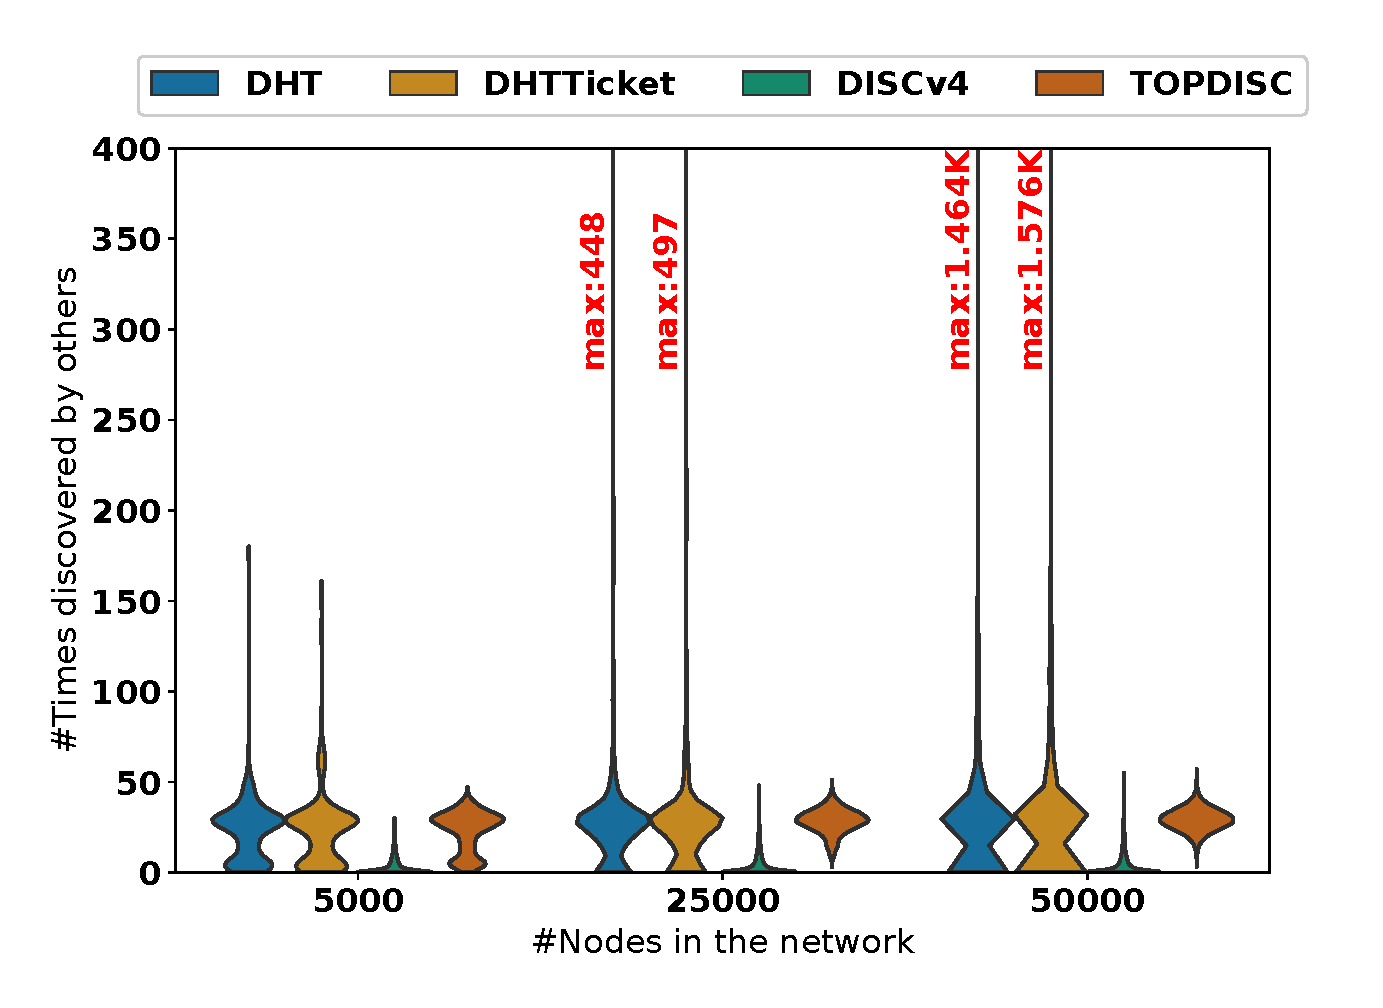
\includegraphics[width=\linewidth]{results/efficiency/violin_size_wasDiscovered.eps}
%\caption{Y-axis: .}
%\label{fig:regsPlacedPerSize}
%\end{figure}
%
%\begin{figure}
%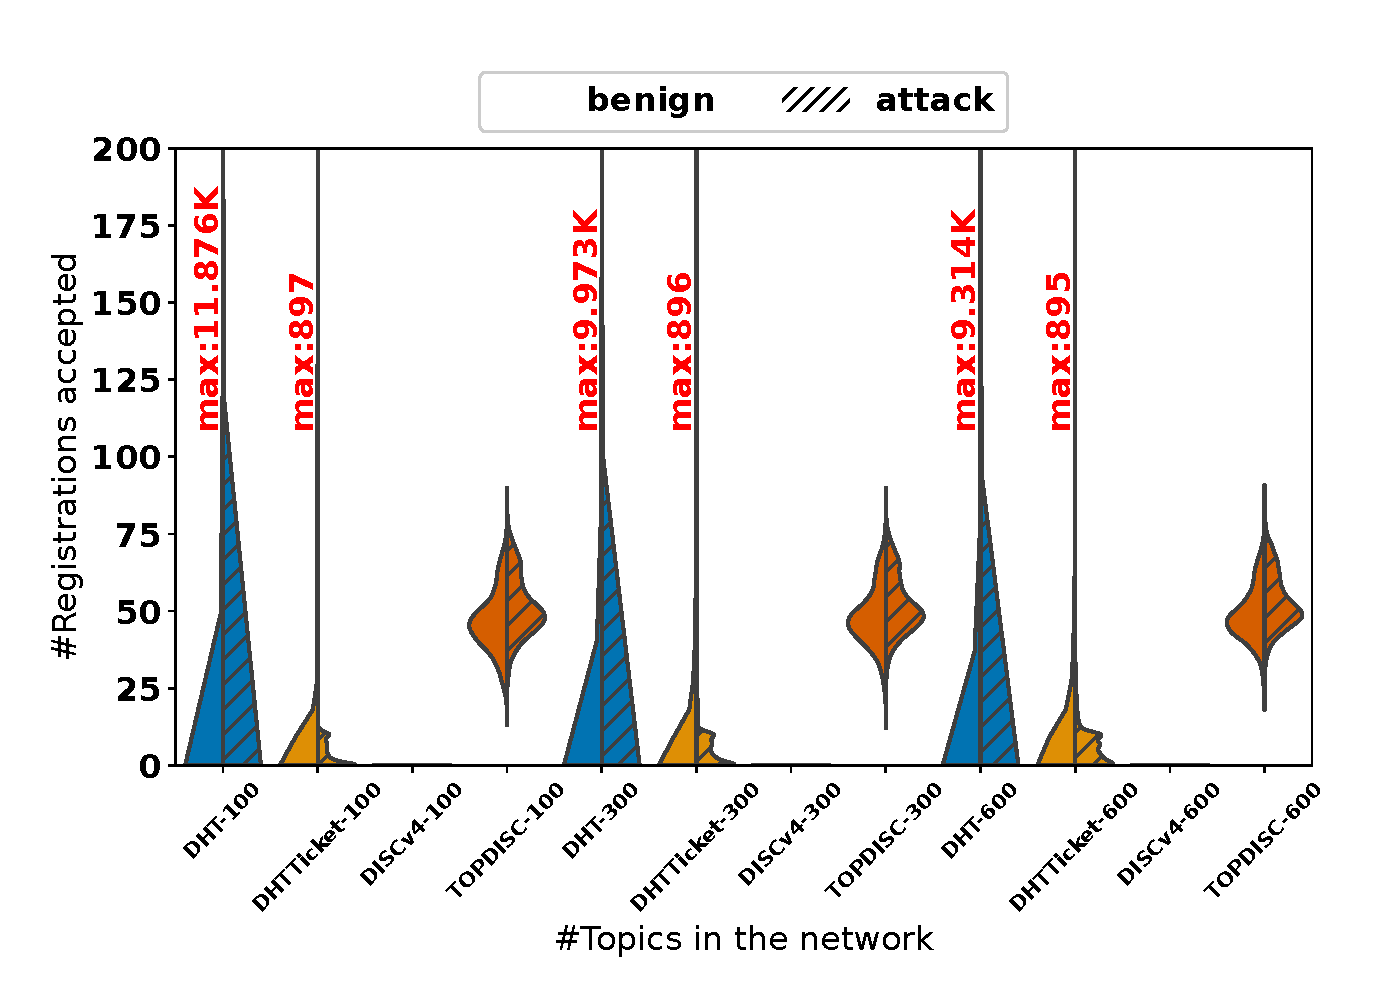
\includegraphics[width=\linewidth]{results/split/topic_regsAccepted.eps}
%%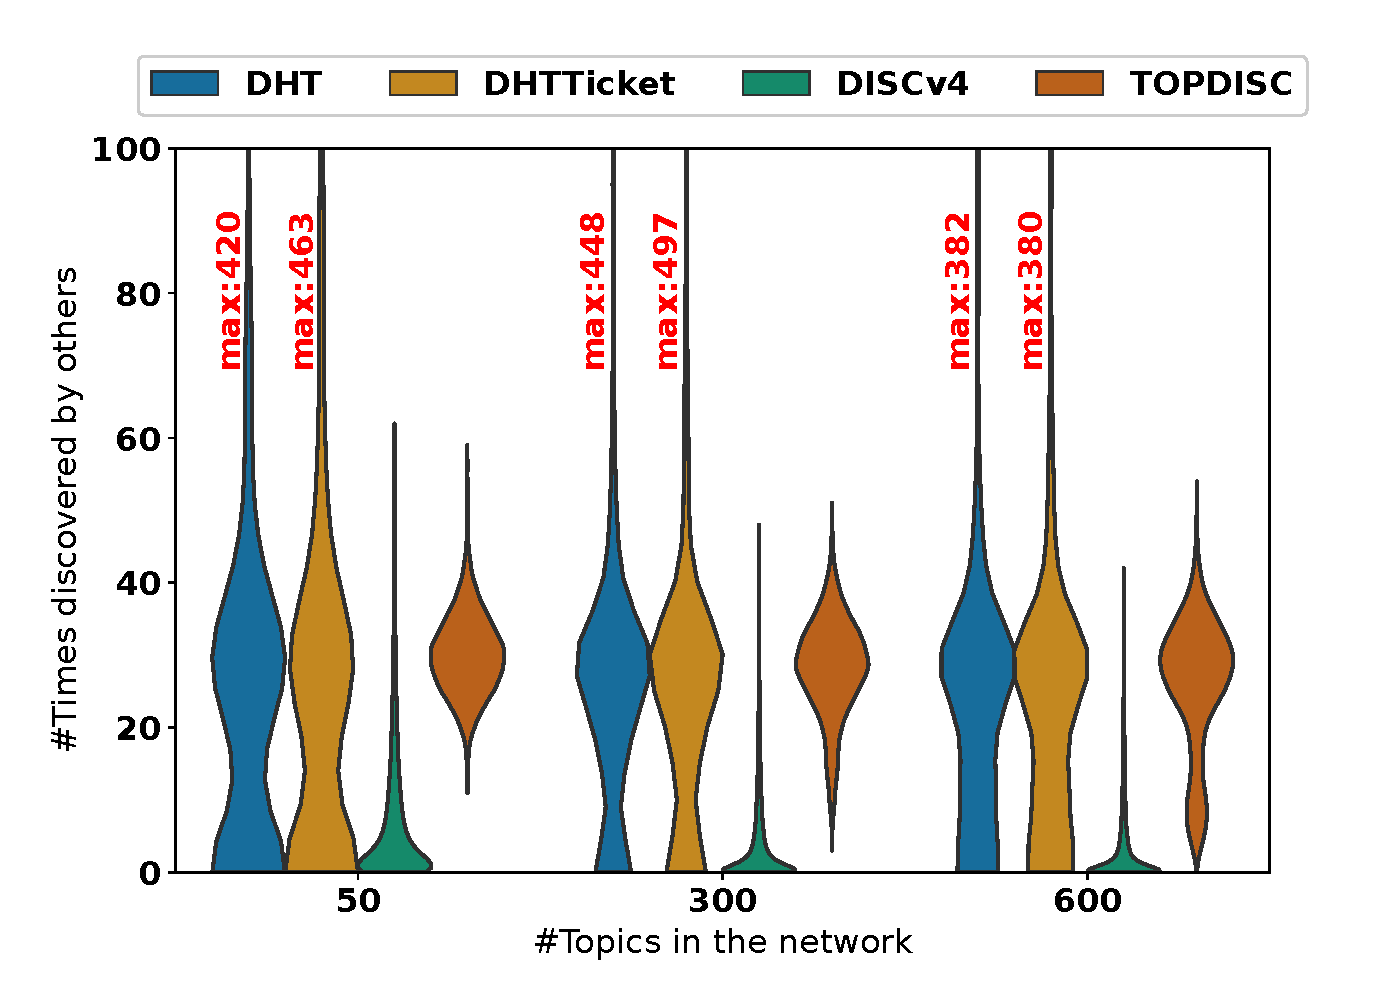
\includegraphics[width=\linewidth]{results/efficiency/violin_topic_wasDiscovered.eps}
%\caption{Y-axis: .}
%\label{fig:regsAcceptedTopic}
%\end{figure}
%
%\begin{figure}[!h]
%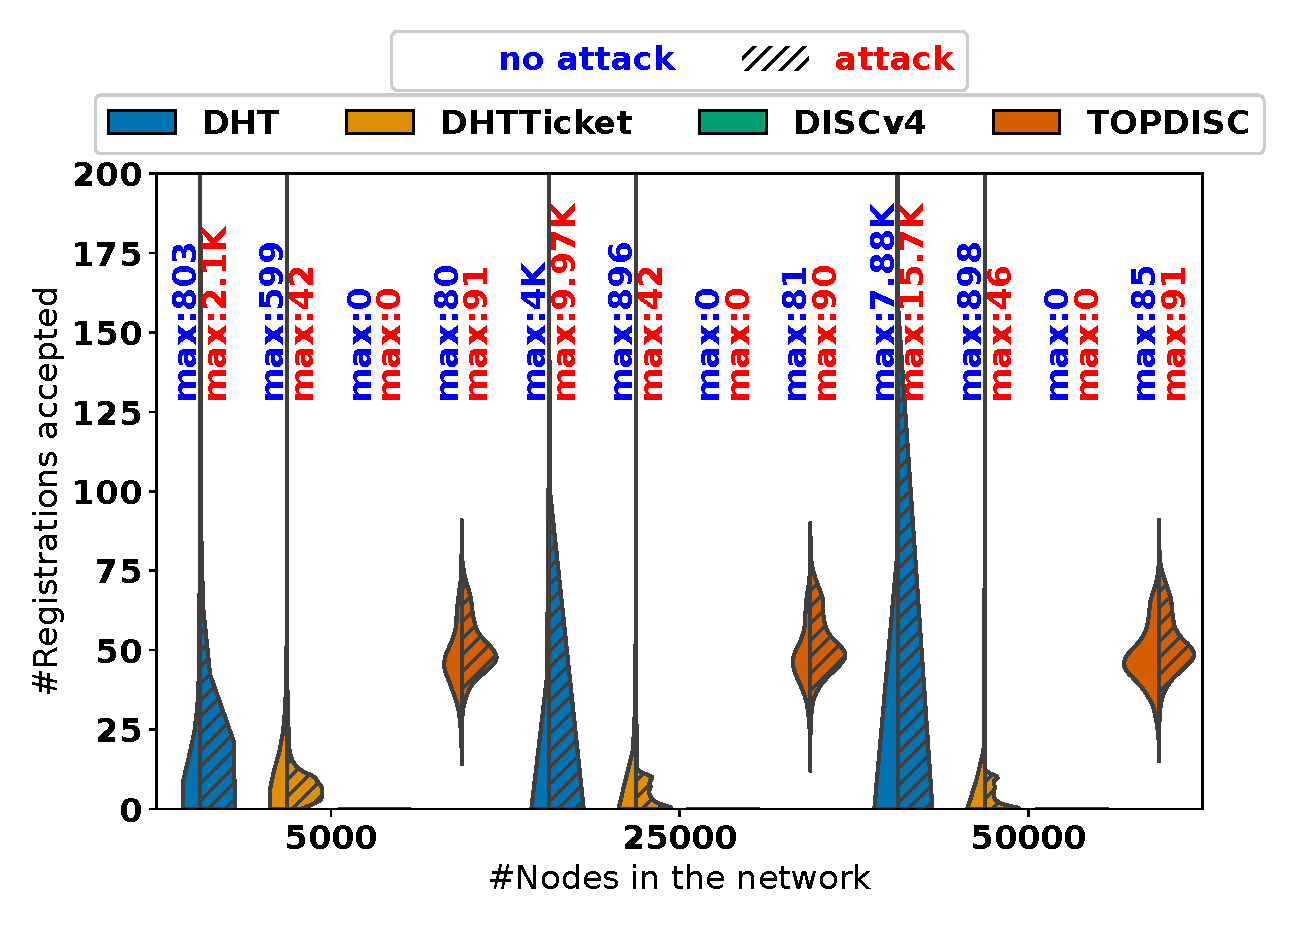
\includegraphics[width=\linewidth]{results/split/size_regsAccepted.eps}
%%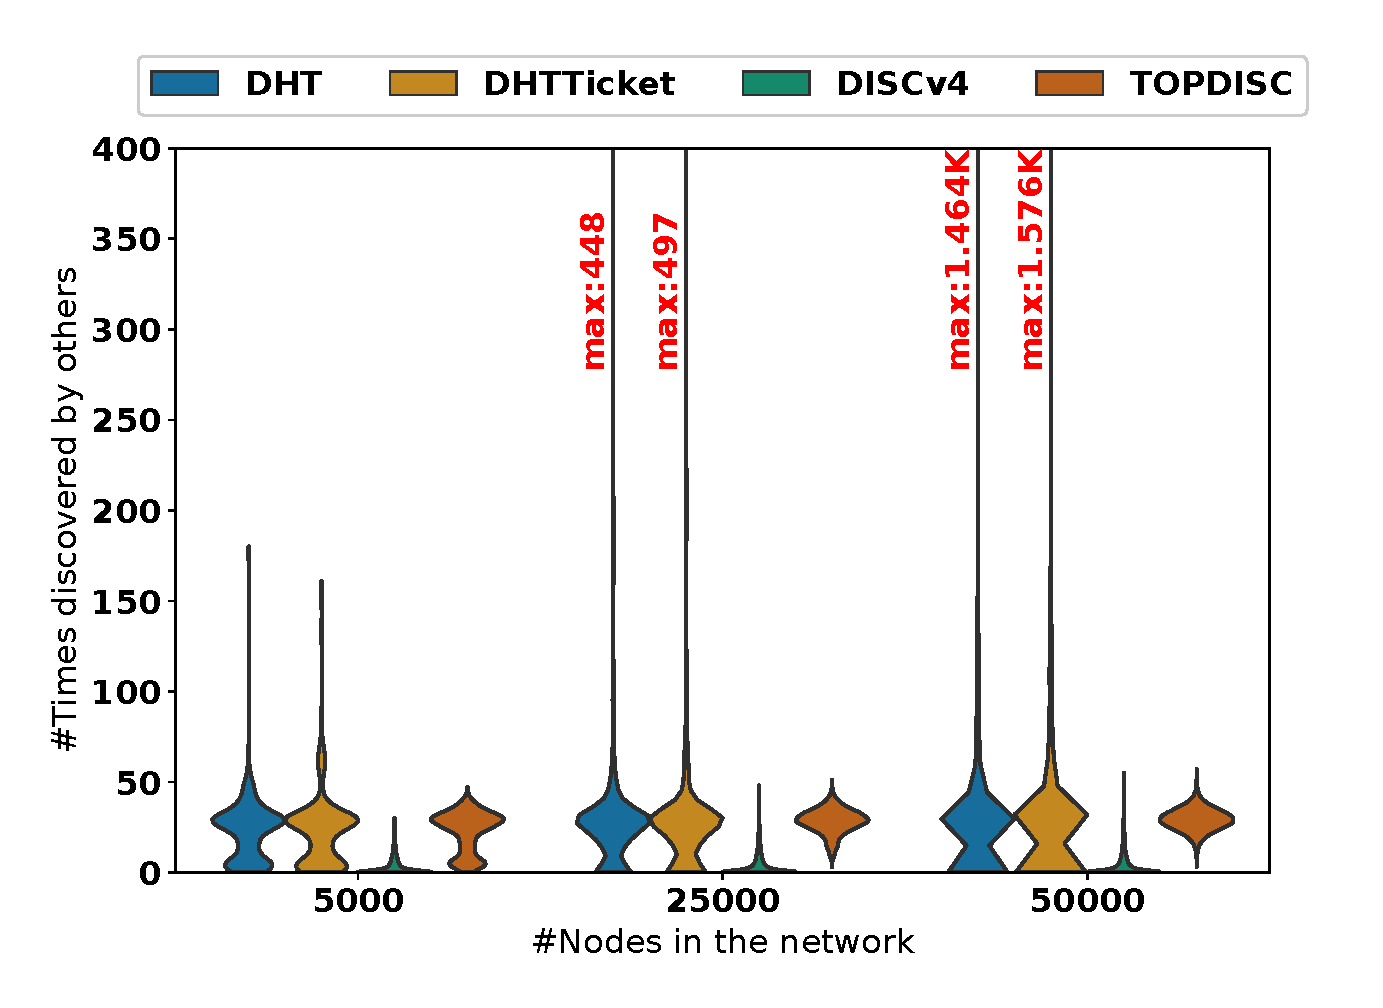
\includegraphics[width=\linewidth]{results/efficiency/violin_size_wasDiscovered.eps}
%\caption{Y-axis: .}
%\label{fig:regsAcceptedSize}
%\end{figure}

%	\subsection{Eclipse attack resistance}
%We evaluate \sysname resistance to two groups of malicious attacks:
%\begin{itemize}
%    \item \textbf{Eclipse Attack} - the attacker tries to make a target node discover and connect to peers under the attacker's control. The attack succeeds when all the inbound and outbound connections of the target node are established with malicious peers. 
%    \item \textbf{Denial of Service (DoS)} - the attacker tries to disturb protocol operations. The attack succeeds when service discovery is made impossible or significantly delayed for a group of benign nodes.  
%\end{itemize}
%The attacker may use a large but finite number of malicious nodes. Both attacks may target a single node or a group of nodes (\eg nodes participating in a specific application). 

%\para{Eclipse Attack}

\para{Eclipse attack resistance}
We evaluate \sysname resistance against eclipse attacks where an attacker simultaneously behaves as a malicious DHT peer, a malicious registrar and a spamming advertiser (see \Cref{sec:threat}). 

In the attack scenarios, we assume a single entity controlling a pool of Sybils that have access to a limited pool of IP addresses. Malicious nodes register ads for the \er{a?} target topic at a rate 10 times higher than that of honest nodes. Malicious nodes return other malicious peers in response to both DHT routing and topic queries. The objective of the attackers is to eclipse as many peers as possible by taking over their (outbound) connections.

The simulations run for one hour and we report results from a single lookup operation per node for the topic it participates to. On top of each violin plot, we specify the \emph{percentage of eclipsed (benign) nodes after a lookup operation}; that is, the percentage of lookups where all the peers obtained are malicious. We assume that the attacker identifiers are uniformly distributed in the address space. We omit the results for scenarios with non-uniform Sybil ID distributions. In that case, the \altname and \altnameticket suffer from $100\%$ eclipse rates. \er{we should probably define eclipse rate more formally before using it, it is a central metric.} With as little as $N_{malicious} = 30$ nodes, an adversary can intercept all the lookup queries for the target topic. At the same time, \sysname is shown to achieve lower eclipse rates under a non-uniform Sybil ID distribution (~\Cref{sec:analysis}). The results below represent the worst-case scenario for \sysname and the best-case scenario for protocols we compare against. 
We evaluate the eclipse attacks targeting two specific topics: the most popular (3978 honest nodes) and the least popular (33 honest nodes) topics.
%We evaluated the attacks for the most popular and least popular 


%\begin{figure}[!h]
%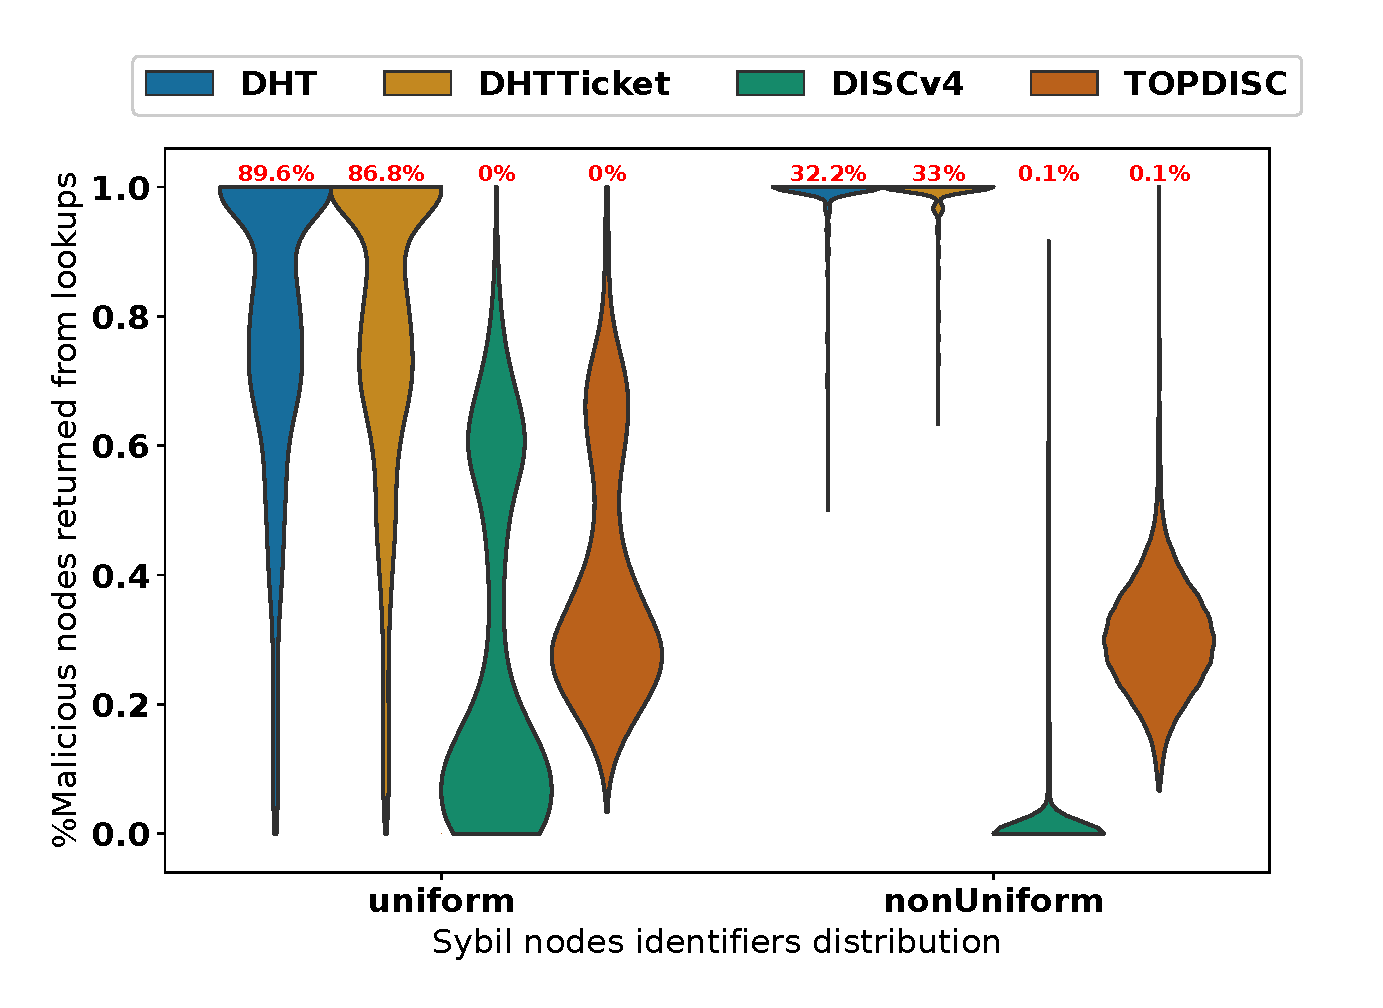
\includegraphics[width=\linewidth]{results/security/violin_idDistribution_percentageMaliciousDiscovered_t0.eps}
%\caption{Y-axis: Malicious nodes discovered and percentage eclipsed nodes using uniform distributed sybil identities vs generating node ids close to topic id,   when attacking the most popular topic (3978 nodes).}
%\label{fig:eclipse_distribution_t0}
%\end{figure}
%
%In Figure~\ref{fig:eclipse_distribution_t0} we show the malicious nodes discovered for all lookups for all protocols using different distribution of the identifiers of the malicious nodes,  when attacking the most popular topic (with 3978 nodes).  In the first option, the malicious nodes ids are artificially generated with a small distance to the topic hash id.  In the second option, malicious nodes identifiers are uniformly distributed.  In the figure we can observe that for \altname and \altnameticket the percentage of eclipses are superior to 80\% because most of the nodes close to topics identifiers are nodes controlled by the attacker.  
%For \altname and \altnameticket, the lookup process is similar to Kademlia lookup process and,  placing all malicious nodes close the topic hash,  it makes very likely to query only malicious nodes during the process, since it only queries the closest known nodes to the topic identifier.
%When attackers are uniformly distributed in the network, eclipses are reduced to close to 32.9\% and 33.7\% respectively.
%Even though it is much less likely to hit malicious nodes during the lookup in this case (remember the default number of malicious are 1000 -4\% of the network-),  when hitting a malicious nodes, the nodes returned by them are used to continue the  query and it may happen it continues querying malicious nodes only during the process.
%When a low popularity topic is attacked (with only 33 nodes),  as shown in Figure~\ref{fig:eclipse_distribution_t299},  for  \altname and \altnameticket the eclipses are even higher, reaching a 100\% of eclipses when placing malicious nodes close to the topic id, and reaching a 78.8\% and 90.9\% when distributing malicious nodes uniformly.  
%Remember the number of attackers is 1000,  against the 33 valid nodes.
%
%For \discv,  the number of eclipses reach is 0\% for the most popular topic when attackers are placed close to the topic hash.  When Sybil nodes are uniformly distributed the number of malicious nodes returned increases,  but to a very low 0.1\%.
%This is caused by the fact that \discv does not target lookups to any specific identifier,  but completely random identifiers,  so it is very difficult for the attackers to place Sybil nodes where they will be queried.  Moreover it is difficult by the attackers to send identifiers where the lookup process will be likely to continue to,  because in the FIND node for the Ethereum DHT the lookup identifier is not disclosed,  but only the distance to it.
%The number of eclipses reach 12.1.\% for the least popular topic when attackers are placed close to the topic hash.  When Sybil nodes are uniformly distributed the number of malicious nodes returned increases,  however the eclipses  reach a 78.8\%.
%The resistance of \discv to Sybil attacks is obtained with the important trade-off of very low efficiency when finding nodes for specific topics, specially for low popular topics.  It is very likely that, when doing lookups using \discv for very low popular topics, no nodes are found or just a few of them.   This means when hitting a malicious node during lookup,  it is likely with a single query to a malicious node, the node querying will be eclipsed.
%
%For \sysname, the number of eclipses are very low for the most popular topic. 
%The eclipses are 0\% when Sybil nodes are placed close to topic id and 0.5\% when are uniformly distributed, with similar distribution to the malicious nodes returned compared with \discv.
%However when attacking the least popular topic the eclipses increase to 78.8\% for both cases.
%This is due to the very low number of valid nodes (33),  that will be more difficult to find than the attackers (1000 nodes, reusing 100 IP addresses).  
%But event the high number of attackers in almost half the cases valid nodes are also found along the evil nodes.
%Remember that Sybil nodes are completely valid nodes from a network discovery point of view when using different network addresses.
%
%\begin{figure}[!h]
%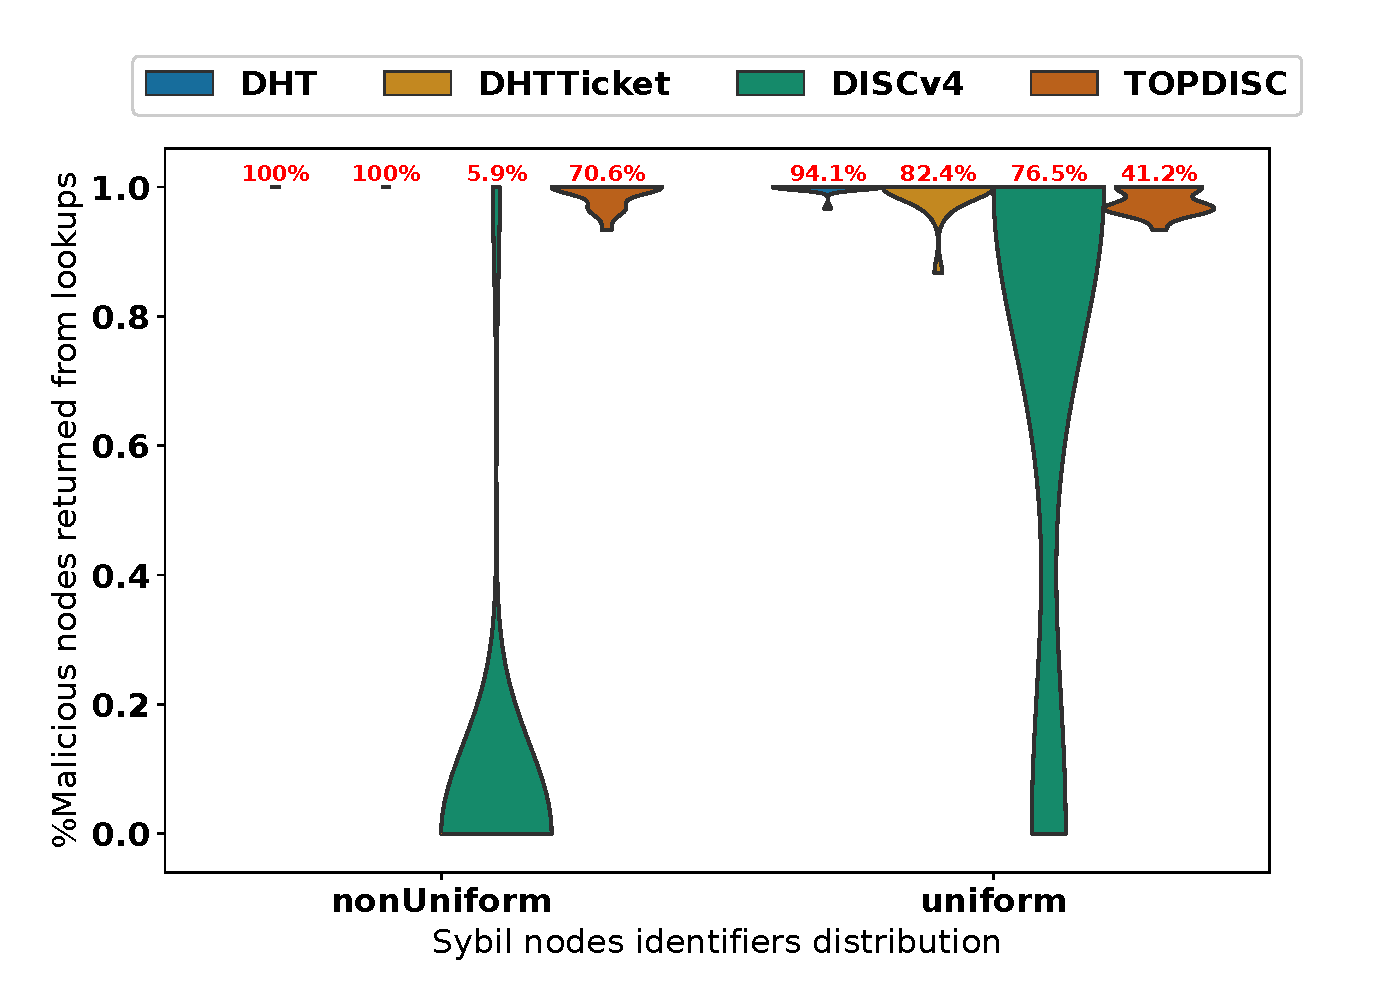
\includegraphics[width=\linewidth]{results/security/violin_idDistribution_percentageMaliciousDiscovered_t299.eps}
%\caption{Y-axis: Malicious nodes discovered and percentage eclipsed nodes using uniform distributed sybil identities vs generating node ids close to topic id,   when attacking the low popularity topic (33 nodes).}
%\label{fig:eclipse_distribution_t299}
%\end{figure}

\Cref{fig:eclipse_evil_t0} and \Cref{fig:eclipse_evil_t299} present the percentage of malicious nodes in the lookup results and the percentage of eclipsed nodes for the most and the least popular topic, respectively.
% In both figures, Sybil nodes use a pool of 100 IP addresses, and we observe the impact of Sybil size on the eclipse resistance of all four mechanisms. 
In \Cref{fig:eclipse_evil_t0}, \discv and \sysname achieve close to a $0$ eclipse rate, even with a high number of malicious nodes. On the other hand, both \altname and \altnameticket have significantly worse performance with respectively 26.7\% and 25.9\% eclipses \er{eclipse rates?} when there are 1000 attackers.
In \Cref{fig:eclipse_evil_t299}, 
when Sybils attack the least popular topic, we observe \sysname to be the most resistant to eclipsing as can be seen in \Cref{fig:eclipse_evil_t299}. \sysname's high resistance to eclipsing even for the least popular topic with a large Sybil presence highlights the effectiveness of both the waiting time mechanism and distributing the lookup and registration operations across different buckets.
 
\begin{figure}[!h]
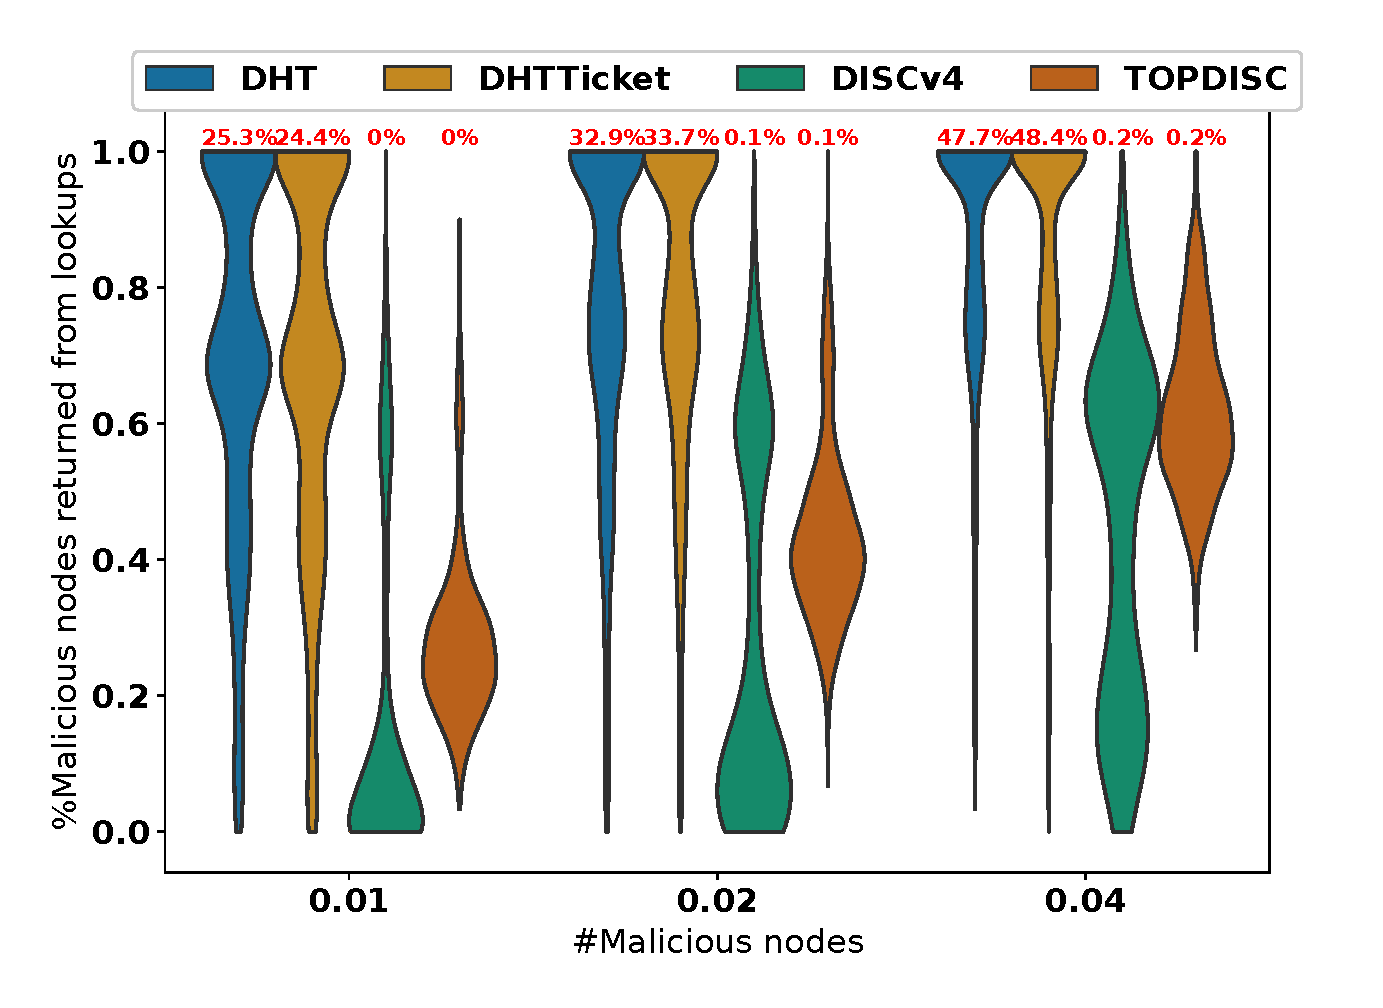
\includegraphics[width=\linewidth]{results/security/violin_percentEvil_percentageMaliciousDiscovered_t0.eps}
\caption{Y-axis: Malicious nodes discovered and percentage eclipsed nodes for a different number of Sybil nodes used in the attack when attacking the most popular topic (3978 nodes).}
\label{fig:eclipse_evil_t0}
\end{figure}

\begin{figure}[!h]
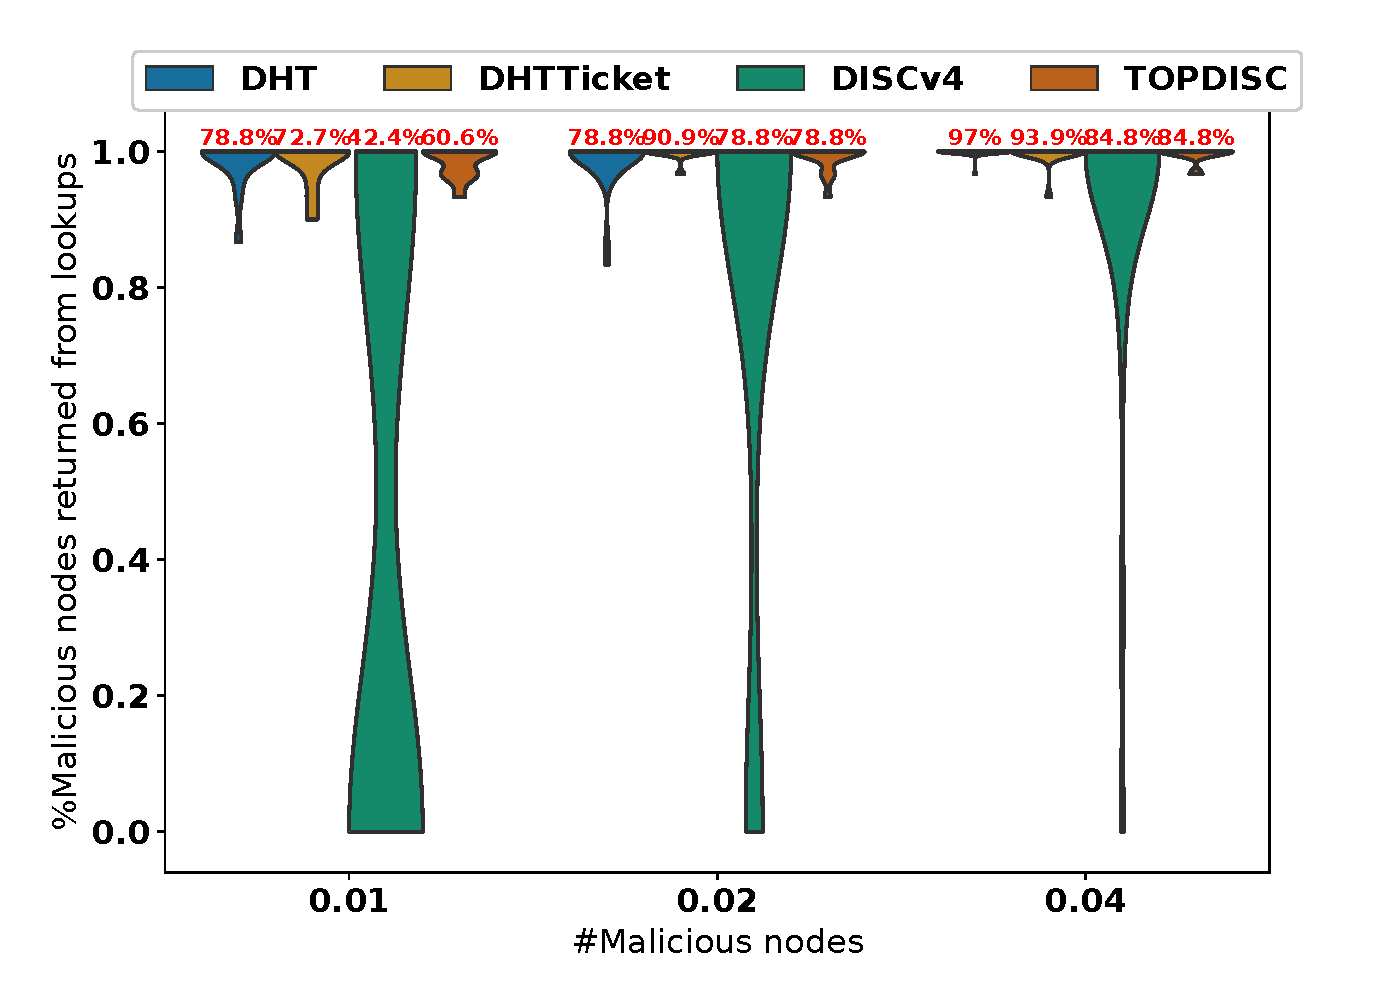
\includegraphics[width=\linewidth]{results/security/violin_percentEvil_percentageMaliciousDiscovered_t299.eps}
\caption{Y-axis: Malicious nodes discovered and percentage eclipsed nodes for a different number of Sybil nodes used in the attack when attacking the least popular topic (33 nodes).}
\label{fig:eclipse_evil_t299}
\end{figure}

In \Cref{fig:eclipse_sybil_t0} and \Cref{fig:eclipse_sybil_t299}, we again illustrate the percentage of malicious nodes in the lookup results and the percentage of eclipsed nodes for the most and the least popular topic, respectively. In these figures, we vary the size of the IP address pool used by the adversary. We observe that both \sysname and \discv achieve close to no eclipsing, while in \altname and \altnameticket at least 30\% of nodes are eclipsed in all cases.
When attacking the least popular topic using 100 IPs, the percentage of eclipsed nodes is similar for all four mechanisms. However, \sysname performs significantly better for a lower number of IP addresses under the control of the adversary.
More specifically, we observe that, when using \sysname, only 5.9\% of nodes are eclipsed when the adversary has a single IP address for its Sybils, which goes up to 41.2\% when 10 IP addresses are used, as opposed to over 70\% of nodes being eclipsed for \discv in all cases.  

\begin{figure}[!h]
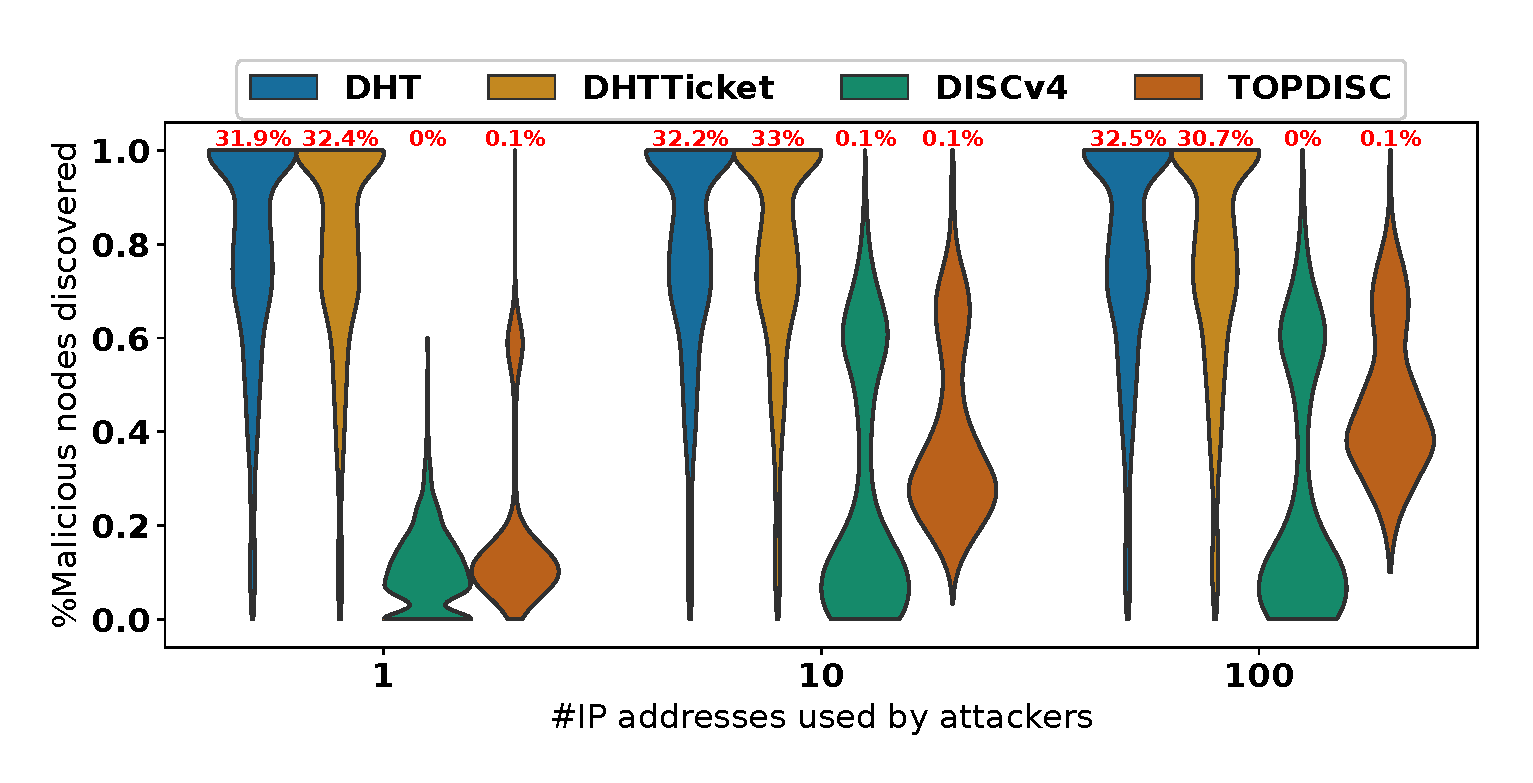
\includegraphics[width=\linewidth]{results/security/violin_sybilSize_percentageMaliciousDiscovered_t0.eps}
\caption{Y-axis: Malicious nodes discovered and percentage eclipsed nodes for different numbers of IP addresses used in the attack when attacking the most popular topic (3978 nodes).}
\label{fig:eclipse_sybil_t0}
\end{figure}



\begin{figure}[!h]
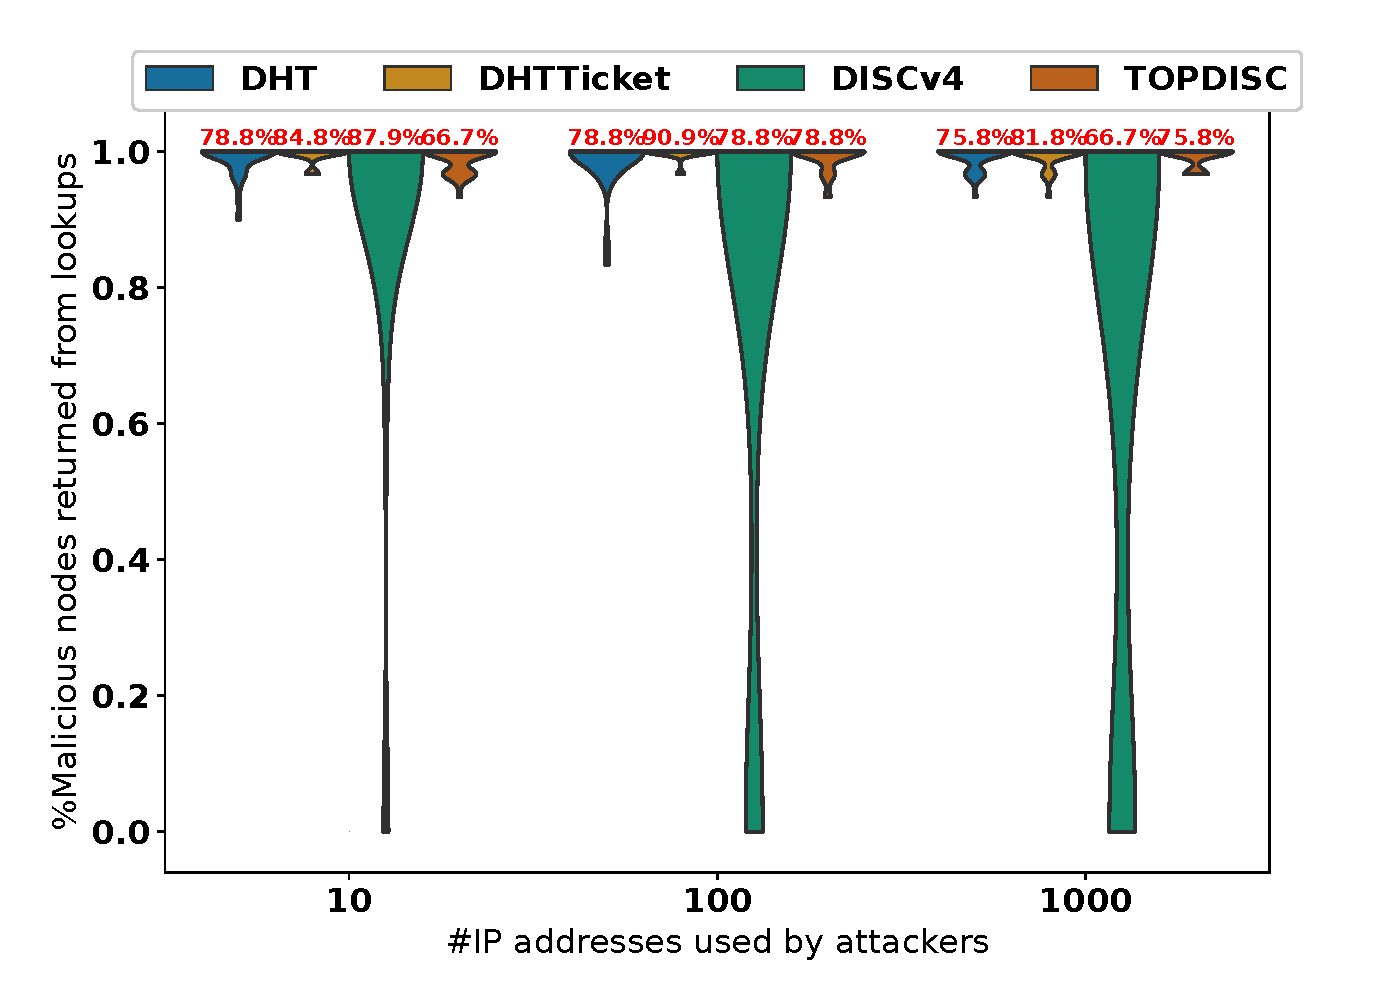
\includegraphics[width=\linewidth]{results/security/violin_sybilSize_percentageMaliciousDiscovered_t299.eps}
\caption{Y-axis: Malicious nodes discovered and percentage eclipsed nodes for different numbers of IP addresses used in the attack when attacking the least popular topic (33 nodes).}
\label{fig:eclipse_sybil_t299}
\end{figure}








%\begin{figure*}[!h]
%\centering
%\subfigure[{Y-axis: Percentage eclipsed nodes using uniform distributed sybil identities vs generating node ids close to topic id}]{
%\includegraphics[width=0.31\textwidth]{results/security/%bar_idDistribution_percentageEclipsedLookups_t0.eps}
%violin_idDistribution_percentageMaliciousDiscovered_t0.eps}
%\label{fig:distribution}
%}
%\subfigure[{Y-axis: Percentage eclipsed nodes for different number of sybil nodes in the attack.}]{
%\includegraphics[width=0.31\linewidth]{results/security/%bar_percentEvil_percentageEclipsedLookups_t0.eps}
%violin_percentEvil_percentageMaliciousDiscovered_t0.eps}
%\label{fig:percentEvil}
%}
%\subfigure[{Y-axis: Percentage eclipsed nodes for different number IP addresses used in the attack.}]{
%\includegraphics[width=0.31\linewidth]{results/security/%bar_sybilSize_percentageEclipsedLookups_t0.eps}
%violin_sybilSize_percentageMaliciousDiscovered_t0.eps}
%\label{fig:sybilsize}
%}
%\caption{Resistance against eclipse attacks when attacking most popular topic (t0)} 
%\label{fig:eclipse_attack}
%\vspace{-0.05in}
%\end{figure*}
%
%\begin{figure*}[!h]
%\centering
%\subfigure[{Y-axis: Percentage eclipsed nodes using uniform distributed sybil identities vs generating node ids close to topic id}]{
%\includegraphics[width=0.31\textwidth]{results/security/%bar_idDistribution_percentageEclipsedLookups_t299.eps}
%violin_idDistribution_percentageMaliciousDiscovered_t299.eps}
%\label{fig:distribution}
%}
%\subfigure[{Y-axis: Percentage eclipsed nodes for different number of sybil nodes in the attack.}]{
%\includegraphics[width=0.31\linewidth]{results/security/%bar_percentEvil_percentageEclipsedLookups_t299.eps}
%violin_percentEvil_percentageMaliciousDiscovered_t299.eps}
%\label{fig:percentEvil}
%}
%\subfigure[{Y-axis: Percentage eclipsed nodes for different number IP addresses used in the attack.}]{
%\includegraphics[width=0.31\linewidth]{results/security/%bar_sybilSize_percentageEclipsedLookups_t299.eps}
%violin_sybilSize_percentageMaliciousDiscovered_t299.eps}
%\label{fig:sybilsize}
%}
%\caption{Resistance against eclipse attacks when attacking least popular topic (t299)} 
%\label{fig:eclipse_attack}
%\vspace{-0.05in}
%\end{figure*}
%\begin{figure}[!h]
%\includegraphics[width=\linewidth]{img/placeholder}
%\caption{Compare only against DHT here I guess? Y-axis a ratio of popular malicious and benign ads in the table for spam attack and topic-targeted attack within a single registrar. X-axis: to avoid showing different graphs for multiple malicious IPs/IDs/nodes we can have a fix ratio between them i.e., each 5 Sybils (or requests/s) have 1 IP and 2 ID, and increase this "attacker strength".} 
%\label{fig:security_spam}
%\end{figure}
%
%\begin{figure}[!h]
%\includegraphics[width=\linewidth]{img/placeholder}
%\caption{Compare only against DHT here I guess? Y-axis a  time to discovery/registration (do we care about registration if lookup works?) slowdown compared to a non-attack scenario?Do we consider different placements of Sybils here (i.e., only bucket 1? Or spread evenly across all the buckets?). X-axis: to avoid showing different graphs for multiple malicious IPs/IDs/nodes we can have a fix ratio between them i.e., each 5 Sybils have 1 IP and 2 ID, and increase this "attacker strength".} 
%\label{fig:security_spam}
%\end{figure}



\iffalse
\subsection{Performance Results}
\michal{We should group the result so that they show achievement of specific goals that we described before}

%\paragraph{Ticket registrations:
In the following we detail the performance evaluation in four different subsections.  In the first we show the registration performance.  Secondly we show the traffic load and overhead of the designed mechanism.  Then we continue with the lookup and discovery performance and we finish with the security analysis.

\subsubsection{Registration  performance}

In Figure~\ref{fig:regs} we observe the average active registrations in the system per topic with different number of nodes in the simulation,  from 500 to 10000 nodes. 
We can observe nodes for all topics are able to place a substantial amount of registrations, even the less popular topics. 
As number of nodes increase in the network, we can observe the differences between registrations per topic are reduced. 
Actually, it can be observed the most popular topic (t1) is able to place less registrations than t2. 
This is caused by the fact that with more nodes trying to register for the same topic,  waiting times increase.
If the waiting time increases over the waiting time limit (in the simulations is set to 15 min),  the node cancels the registration and tries with a different nodes.
When cancellations happen it may lead to less active registrations, because it may end up with longer registration processes.
In our simulation we observe less registrations for t1 than t2  because t1 registrations waiting time go over the waiting time limit more often.

In Figure~\ref{fig:time_reg} we observe the average time necessary for a node to place a registration,  from 500 to 10000 nodes in the simulation.
We can observe that average registration time is always below 500 seconds and this is reduced for less popular topics and smaller networks. 
This figure does not include registration times for cancelled registrations.
\sergi{I think we should include failed/uncomplete registrations in the plot}

\begin{figure}[!h]
\centering
\subfigure[{Active registrations}]{
\includegraphics[width=0.225\textwidth]{img/eval/registration_origin.eps}
\label{fig:regs}
} 
\hspace{-0.25cm}
\subfigure[{Time to register}]{
\includegraphics[width=0.225\textwidth]{img/eval/avg_time_register.eps}
\label{fig:time_reg}
}
 \caption{Ticket registrations} 
\label{fig:registrations}
\vspace{-0.15in}
\end{figure}   

%\begin{figure}[h!]
%\centering
%%\epsfig{file=imgs/eval/scen5.pdf, width=0.45\textwidth}
%\includegraphics[width=0.225\textwidth]{img/eval/registration_origin.png}
%\caption{Registrations}
%\label{fig:regs}
%\vspace{-0.15in}
%\end{figure}

%\paragraph{\bf{Network load}:}
\subsubsection{Network load}

In Figure~\ref{fig:messages}~and~\ref{fig:msg_distr} we can observe the traffic load generated in the network.
In Figure~\ref{fig:messages} we observe most of the messages are ticket requests/replies, and the subsequent registration request/replies
after receiving a ticket from a node. 
This is caused by the fact that nodes are constantly registering dynamically. 
In Figure~\ref{fig:msg_distr} the messages received distribution. 
We can observe some nodes receive much more messages.
This is caused by the bucket node distribution, where nodes with identifiers close to topic hash ids receive more initial tickets requests because there are less.
However, we observe while the number of nodes in the network is increased 20 times,  the  maximum number of messages received by some nodes does not increase in the same way,  only being twice the amount when comparing 500 with 10000 nodes,  ans with increases lower than 30\% when number of nodes are doubled.
Moreover,  we can also see the number of messages received does not exceed 10 times the average value of the messages received. 

Therefore, the system is able to scale without danger of overloading some of the nodes of the network.

\begin{figure}[!h]
\centering
\subfigure[{Number of messages}]{
\includegraphics[width=0.225\textwidth]{img/eval/message_quantity.eps} 
\label{fig:messages}
} 
\hspace{-0.25cm}
\subfigure[{Message distribution}]{
\includegraphics[width=0.225\textwidth]{img/eval/messages_received.eps} %\hspace{-1.5em}%
\label{fig:msg_distr}
}
 \caption{Traffic load} 
\label{fig:traffic}
\vspace{-0.15in}
\end{figure}   

\subsubsection{Discovery and lookup performance}

%\paragraph{\bf{Discovery performance}:}

In Figure~\ref{fig:reg_disc} and \ref{fig:timedisc} we can observe how nodes are discovered within the network.
In Figure~\ref{fig:reg_disc} we observe the percentage of the nodes in the network that are discovered and how often are discovered.
Each node in the network is represented by a circle, and the size of the circle represents the relative frequency of discoveries compared with other nodes in the network.
We can observe that for all topics the percentage of nodes discovered in the network is very close to 100\%. This means almost all nodes in the network are able to be discovered by other nodes. The number of discovered nodes is not 100\% because of the existence of turbulence (there are some nodes just joined the network and there has not been enough time yet to be discovered). In case there are a low number of nodes for a specific topic (e.g. t5 with 500 nodes network) the 100\% is reached.
We can also observe Figure~\ref{fig:reg_disc} that the discovery distribution is bounded to \hl{X} times between the most discovered and the least discovered.
We observe the dots size are very regular and despite being not completely equal the differences are not substantial. 
In Figure~\ref{fig:timedisc} we observe the time between a registration is completed and the first time the registration
is returned in a lookup.
By observing this we can see how difficult is for a node to be discovered once is able to place a registration. 
We see the average time is between 20 and 10 seconds in most of the cases, except for the least popular topic t5 which is around 50\% higher. 
We also observe the deviation is bounded at around 60 seconds, with equivalent different for t5.


\begin{figure}[!h]
\centering
\subfigure[{Advertiser discovery distribution}]{
\includegraphics[width=0.225\textwidth]{img/eval/registrant_distribution.eps} 
\label{fig:reg_disc}
} 
\hspace{-0.25cm}
\subfigure[{Time between registration and first discovery}]{
\includegraphics[width=0.225\textwidth]{img/eval/min_time_discovery.eps} %\hspace{-1.5em}%
\label{fig:timedisc}
}
 \caption{Discovery performance} 
\label{fig:discovery}
\vspace{-0.15in}
\end{figure}   


In Figure~\ref{fig:hopcount} we can observe the lookup performance of \sysname compared with Discv4 for a 5000 nodes simulation.
In the plot we show the average number of nodes discovered for each hop during a lookup per topic, taking into account that Discv4 cannot do per topic lookups,  so we discard received nodes that do not support the specific service.
In the figure we observe that for t1 the discovered nodes are higher when using Discv4, since all topics support t1 and any node discovered will be a valid node. 
However, as the popularity of the topic decreases it also does the lookup performance of Discv4,  since it is very difficult to find nodes for non-popular topics without supporting per topic lookups.
In this sense,  Discv5 lookup performance also decreases the performance with non-popular topics (simply because there are less nodes in the network) however this decrease is diminished.  Between t1 and t5 the lookup performance is decrease approximately to a 1/2th for Discv5, while when using Discv4 the lookup performance decreased to a less than a 1/10th.

%TODO add lookup description including mechanisms to avoid sybils.

\begin{figure}[h!]
\centering
%\epsfig{file=imgs/eval/scen5.pdf, width=0.45\textwidth}
\includegraphics[width=0.35\textwidth]{img/eval/lookup_hopcount_discv4.png}
\caption{Lookup performance}
\label{fig:hopcount}
\vspace{-0.15in}
\end{figure}

\subsubsection{Sybil Attacks}

In the following we show the results of the performance evaluation of the discovery service under different sybil attacks.  The attacks that we evaluated in this section are of two types and are previously described in Section~\ref{sec:overview}. 
These attacks are eclipsing  and Denial-of-service (DoS) attacks.
Eclipsing attacks goal is to generate multiple fake identities within a topic to be able to eclipse existing nodes in the network.
Eclipsing a node imply all outbound and inbound connections are established to only sybil/fake nodes controlled by an attacker.
This allows the attacker to control the view of the network of the eclipsed node and can be used to co-opt a victim's mining power and use it to attack the blockchain's consensus algorithm.
DoS attacks instead is an attack meant to hamper the good performance or even to shut down the network, making it inaccessible to its intended users.  
In our case,  the goal of DoS attacks is to difficult or to block the discovery of nodes in the network and is specially important for topic with low popularity where finding all node in the network is very important.

In the implemented topic eclipsing attack,  malicious nodes are sybil nodes that cooperate in order to eclipse other valid nodes.
Malicious and valid nodes have the same amount of bandwidth resources and malicious nodes respond to topic lookup requests and find messages with only other malicious nodes.
Malicious nodes also act as evil 'advertisers' trying to place as many registrations as possible by using bigger ticket size,  with malicious registrars attack,  where evil registrars replies with only malicious nodes when receiving a topic query.

We implemented and evaluated two kind of DoS attacks.  
The first attack consists in a topic spam attack where a big number of sybil identities generated try to register for non-existing random topics.
By registering for non-existing topics,  evil nodes try to harm valid topics registrations, overflowing ad caches.
The second DoS attack consists on generating sybil identities that keep without replying when receiving valid nodes ticket requests or return very long waiting times. 
This way an attacker can try to backlog valid nodes ticket registrations.

In Figures~\ref{fig:reg_eclipse},~\ref{fig:discoverytime_eclipse}~and~\ref{fig:lookup_eclipse} we show performance results under a
topic eclipsing attack.
We compare results for topic eclipsing attacks targeted to the most popular topic (t1) and attacks targeted to the least popular topic (t5). 
In the simulation there are 2000 nodes, all of them participating in t1 and only 218 participating in t5. 
In the simulations there are an additional 20\% (400 in total) malicious nodes that target the specific topic and the number of resources used in the attack (IP addresses) vary from 1 address to 50.

\begin{figure}[!h]
\centering
\subfigure[{Active registrations eclipse attack t1 attack}]{
\includegraphics[width=0.22\textwidth]{img/eval/attack/registration_origin_t1.eps} 
\label{fig:reg_eclipse_t1}
} 
\hspace{-0.15cm}
\subfigure[{Active registrations eclipse attack t5 attack}]{
\includegraphics[width=0.22\textwidth]{img/eval/attack/registration_origin_t5.eps} %\hspace{-1.5em}%
\label{fig:reg_eclipse_t5}
}
 \caption{Active registrations under topic eclipsing attack} 
\label{fig:reg_eclipse}
\vspace{-0.15in}
\end{figure}   

In Figure~\ref{fig:reg_eclipse_t1} we observe the active registrations in the simulation per topic, for an eclipsing attack targeted to the most popular topic (t1), including active registrations of malicious nodes.
We can observe than even though the number of malicious nodes is equivalent to 20\%, the number of active registrations is lower than that. 
As expected, as the number of IP addresses used in the attack increaseas, the number of active registrations of malicious nodes also increase, since different malicious nodes with complete different IPs can not be diffierentiated from valid nodes.
For topic 5, the most vulnerable topic for being the least popular, we can observe a similar pattern of active registrations. 
However, we observe that despite malicious nodes being more (400 nodes) than valid nodes (218 nodes), active registrations of malicious nodes is kept lower than 30\% in all cases. Similarly to t1, the active registrations increase with the higher number of IPs used in the attack, since there is no way to a totally distributed attack without reusing IP addresses.


\begin{figure}[!h]
\centering
\subfigure[{Time between registration and first discovery t1 attack}]{
\includegraphics[width=0.225\textwidth]{img/eval/attack/min_time_discovery_t1.eps} 
\label{fig:discoverytime_eclipse_t1}
} 
\hspace{-0.16cm}
\subfigure[{Time between registration and first discovery t5 attack}]{
\includegraphics[width=0.225\textwidth]{img/eval/attack/min_time_discovery_t5.eps} %\hspace{-1.5em}%
\label{fig:discoverytime_eclipse_t5}
}
 \caption{Time between registration and first discovery under topic eclipsing attack} 
\label{fig:discoverytime_eclipse}
\vspace{-0.15in}
\end{figure}   

In Figure~\ref{fig:discoverytime_eclipse} we observe the average time between a node registers for a topic successfully and the node is discovered for the first time from the placed registration.
We can observe that when a topic is under attack the time required for first time discovery increases. 
This is caused by the fact that there are much more registrations in the topic caused by the attack and also that malicious nodes discovery time is higher due to the difficulty to place registrations in nodes close to the topic hash.  
We can observe that when using more IP addresses in the attack the time required to discover a node is reduced because malicious nodes are more discovered.

\begin{figure}[!h]
\centering
\subfigure[{Lookup hopcount eclipse attack t1}]{
\includegraphics[width=0.225\textwidth]{img/eval/attack/lookup_hopcount_t1.eps} 
\label{fig:lookup_eclipse_t1}
} 
\hspace{-0.16cm}
\subfigure[{Lookup hopcount eclipse attack t5}]{
\includegraphics[width=0.225\textwidth]{img/eval/attack/lookup_hopcount_t5.eps} %\hspace{-1.5em}%
\label{fig:lookup_eclipse_t5}
}
 \caption{Lookup hopcount under topic eclipsing attack} 
\label{fig:lookup_eclipse}
\vspace{-0.15in}
\end{figure}   

%\sergi{redo fig14 and fig15 figures increasing font and using eps}

In Figure~\ref{fig:lookup_eclipse} we observe the lookup hopcount in the simulation per topic,  for an eclipsing attack targeted to the most popular topic (t1) and the least popular topic (t5).
We observe that despite receiving an attack targeted at a specific topic,  the lookup performance in the network is not substantially affected by the attack.

In Figure~\ref{fig:perf_spam} we observe the performance of the topic discovery system under  the topic spam attack.
\sergi{TODO: add no sybil in the graph}
In Figure~\ref{fig:active_regs_spam} we observe the average active registrations per topic increasing the number of IP addresses used by sybil identities performing the attack.  
We observe that the number of active registrations per topic are decreased under the topic spam attack being topic 1 the most affected.
However, by observing Figure~\ref{fig:hopcount_spam} we see he lookup performance is not affected and therefore there is no substantial impact of the attack in the discovery performance of the network, concluding the system is resistant to topic spam attacks.
In Figure~\ref{fig:time_register_spam} we observe the average time required for registering for a topic,  increasing the number of Ip addresses used by sybil identities performing the attack.  
We observe again it seems there is no substantial impact of the attack to the time required to register for each topic

\sergi{add spam storage used?}

\begin{figure*}[!h]
\centering
\subfigure[{Active registrations under topic spam attack}]{
\includegraphics[width=0.275\textwidth]{img/eval/attack/registration_origin_spam.png} 
\label{fig:active_regs_spam}
} 
\hspace{-0.16cm}
\subfigure[{Time to register under topic spam attack}]{
\includegraphics[width=0.275\textwidth]{img/eval/attack/avg_time_register_spam.png} %\hspace{-1.5em}%
\label{fig:time_register_spam}
}
\hspace{-0.15in}
\subfigure[{Lookup hop count topic spam attack}]{
\includegraphics[width=0.275\textwidth]{img/eval/attack/lookup_hopcount_spam.png} %\hspace{-1.5em}%
\label{fig:hopcount_spam}
}
\caption{Performance evaluation topic spam attack} 
\label{fig:perf_spam}
\vspace{-0.15in}
\end{figure*}   

In Figure~\ref{fig:perf_dos} we observe the performance of the topic discovery system under the dos attack where registrars do not respond to advertisers trying to block active registrations.
In Figure~\ref{fig:active_regs_dos} we observe the average active registrations per topic increasing the number of sybil identites from 5\% to 20\% of the nodes in the network.
We observe that the number of registrations are affected by attackers,  being more affected for very popular topics,  but less affected low popularity topics.  However in none of the cases malicious nodes are able to block the active registrations and the reduction of the performance is lower than the number of sybils used.
In Figure~\ref{fig:time_register_dos} we observe the average time required for registering for a topic,  increasing the number of sybil identites from 5\% to 20\% of the nodes in the network.
We observe in this case it seems there is no substantial impact of the attack to the time required to register for each topic
In Figure~\ref{fig:time_discovery_dos} we observe the average time between an advertiser place a registration in a registrar and another node discovers it through the registrar,  increases the number sybils again.
We also observe there is no substantial impact of the attack, concluding the system is resistant to DoS attacks.

\begin{figure*}[!h]
\centering
\subfigure[{Active registrations under DoS attack}]{
\includegraphics[width=0.275\textwidth]{img/eval/attack/registration_origin_dos.png} 
\label{fig:active_regs_dos}
} 
\hspace{-0.16cm}
\subfigure[{Time to register under DoS attack}]{
\includegraphics[width=0.275\textwidth]{img/eval/attack/avg_time_register_dos.png} %\hspace{-1.5em}%
\label{fig:time_register_dos}
}
\label{fig:discovery_dos}
\hspace{-0.15in}
\subfigure[{Time to first discovery under DoS attack}]{
\includegraphics[width=0.275\textwidth]{img/eval/attack/min_time_discovery_dos.png} %\hspace{-1.5em}%
\label{fig:time_discovery_dos}
}
\label{fig:perf_dos}
\caption{Performance evaluation no-response DoS attack} 
\vspace{-0.15in}
\end{figure*}   

\fi
%\subsection{Testbed evaluation}
%
%"Geth"~\cite{go-ethereum} performance evaluation: \hl{TBC}.
